%&&&&&&&&&&&&&&&&&&&&&&&&&&&&&&&&&&&&&&&&&%
%% Übungsblattvorlage					  %
%%% written by Andreas Rain				  %
%&&&&&&&&&&&&&&&&&&&&&&&&&&&&&&&&&&&&&&&&&%

\documentclass[fleqn, oneside, 10pt, titlepage]{report}
%
%Zeichensatz UTF-8 und T1-Zeichensatz
\usepackage[utf8x]{inputenc} 
\usepackage[T1]{fontenc}
%\newcommand{\changefont}[3]{\fontfamily{#1}\fontseries{#2}\fontshape{#3}\selectfont}
% 

%Silbentrennung nach neuer deutscher Rechtschreibung
%\usepackage[ngerman]{babel} % Neue Rechtschreibung
%
%Einige Mathe-Symbole aus AMS-LaTeX
\usepackage{amsmath,amssymb,euscript}
%
% schönere Aufzählungen
\usepackage{enumerate}
%
% Für Bilder 
\usepackage{graphicx}
\usepackage{float} % lädt das Paket zur Verwendung von zusätzlichen Positionsbefehlen

%Graue box
\usepackage{framed}
\usepackage{xcolor}

\definecolor{MyBoxColor}{rgb}{0.9,0.9,0.9}
\newenvironment{shadedSmaller}{
  \def\FrameCommand{\fboxsep=\FrameSep \colorbox{MyBoxColor}}
  \MakeFramed {\advance\hsize-2\width\FrameRestore}}
{\endMakeFramed}

\newenvironment{shadedSmallerPadding}{
  \def\FrameCommand{\fboxsep=0.3cm \colorbox{MyBoxColor}}
  \MakeFramed {\advance\hsize-1.1\width\FrameRestore}}
{\endMakeFramed}
%%%%%%%%%%%%%%%%%%%%%%%%%%

% Standard Font auf Überschriften übernehmen.
%\usepackage{sectsty}
%\sectionfont{\fontfamily{pag}\fontseries{b}\fontsize{13pt}{20pt}\selectfont}
%\subsectionfont{\fontfamily{pag}\fontseries{b}\fontsize{11pt}{20pt}\selectfont}
%\subsubsectionfont{\fontfamily{pag}\fontseries{b}\fontsize{10pt}{20pt}\selectfont}
%\paragraphfont{\fontfamily{pag}\fontseries{b}\fontsize{11pt}{20pt}\selectfont}
%\subparagraphfont{\fontfamily{pag}\fontseries{b}\fontsize{10pt}{20pt}\selectfont}

%
% Farben und die Code-Umgebung einbinden
%
\usepackage{listings, color}
%
% Ein paar Standardfarben
\definecolor{darkblue}{rgb}{0,0,.6}
\definecolor{darkred}{rgb}{.6,0,0}
\definecolor{darkgreen}{rgb}{0,.6,0}
\definecolor{red}{rgb}{.98,0,0}
%
%Standardmäßig Java vorher laden
\lstloadlanguages{Java}
\lstloadlanguages{SQL}
% Standard-Layout für die Code-Umgebung (alle Sprachen)
\lstset{%
	language=SQL,
 	basicstyle=\footnotesize\ttfamily,
	showspaces=false,
	showtabs=false,
	columns=fixed,
	frame=none,
	numberstyle=\tiny,
	breaklines=true,
	showstringspaces=false,
	xleftmargin=0cm,
	tabsize=4,
	keywordstyle=\color{darkblue},
	commentstyle=\color{darkred},
	stringstyle=\color{darkgreen},
	emph={i, t, a, f},
	emphstyle=\color{red}
}%

% New commands for matrices
\newcommand{\rectmat}[1]{\left[\begin{matrix}#1\end{matrix}\right]}
\newcommand{\roundmat}[1]{\left(\begin{matrix}#1\end{matrix}\right)}
\setcounter{MaxMatrixCols}{20}

%
% Seitenranddefinitionen
%   Links etwas mehr Rand als rechts, damit sich die Zettel später besser abheften lassen.
\usepackage[a4paper]{geometry} 
\geometry{a4paper,tmargin=2.5cm, bmargin=3cm, lmargin=3cm, rmargin=3cm, headheight=3em, headsep=1em, footskip=1cm} 

%
% Kopf- und Fußzeilendefinition
%
\usepackage{fancyhdr}
\pagestyle{fancy}
\fancyhf{}
%


% Oben rechts die Namen der Teilnehmer der Gruppe
%
%Oben Links das Fach und darunter die Nummer des Übungsblattes
\fancyhead[L]{\textcolor{gray}{IACV Summary}}
%
% Die Übungsgruppe oben in der Mitte (momentan auskommentiert)
%\fancyhead[C]{Gruppe 2}
%
%Fußzeile mittig die Seitenzahl
\fancyfoot[C]{\textcolor{gray}{Seite \thepage}}
%
% Fußzeile links das aktuelle Datum (alternativ kann hier der Abgabetag eingetragen werden)
\fancyfoot[L]{\textcolor{gray}{\today}}

%Fancy Table
\usepackage{tabularx}
\usepackage{booktabs}
\usepackage{colortbl}
\usepackage{tikz}
\usetikzlibrary{calc}
\pgfdeclarelayer{background}
\pgfdeclarelayer{foreground}
\pgfsetlayers{background,main,foreground}
%

%
% Deutsche Absatzformatierung: Zwischen zwei Absätzen eine Zeile (1em) frei und 
% kein Einrücken der ersten Zeile
%
\setlength{\parskip}{1em}
\setlength{\parindent}{0pt}

%Titelseite
\title{\Large IACV Summary}


%
% Beginn des Dokumentes
%
\begin{document}
\chapter*{Introduction}

Note on terminology:

\begin{description}
    \item[Image Analysis] Low to mid level, early vision (Image processing/enhancement, Image segmentation, depth, motion, features)
    \item[Computer Vision] High level, scene interpretation (Models: 3D, Texture, Lighting; Recognition: Objects, activities..)
\end{description}

Summary:

\begin{itemize}
    \item CV deals with difficult inverse problems
    \item Many different cues about a scene in images
    \item Emulate human gain information
    \item Human perception of visual illusions gives deep insight
    \item IA investigate images on low level, to feed information into high level algos.
\end{itemize}
\chapter{Image Filtering}

\section{Image Types and Discretization}

Definition of continuous grey-scale image: \emph{Mapping f from a rectangular domain $\Omega = (0,w) \times (0,h)$ to a co-domain $\mathbb{R}$, $f : \mathbb{R}^2 \supset \Omega \rightarrow \mathbb{R}$}, $\Omega$ is called image domain/plane and $\mathbb{R}$ specifies grey value.

\textbf{Sampling}

Sampling $\Omega$ gives $(f_{i,j})_{i=1,\dots ,N, j=1, \dots , M}$, $i,j$ being pixel elements. Coarse sampling leads to bad image quality (LS 1.6).

Low sampling rates create \textit{aliasing}, i.e., signals are indistinguishable when sampled. From DSP we know that sampling rate has to be greater than nyquist rate (highest frequency in domain).

\textbf{Quantisation}

Discretization of co-domain, i.e., grey value, for instance $\{0,1,...,255\}$ encoded by a byte. Visualization depicted in LS 1.9.

\textbf{m-Dimensional images}

Domain is now $\mathbb{R}^m$, m=1: Signals, m=2: 2D images, m=3: 3D images.

\textbf{Vector-valued images}

I.e., three channel RGB images (color images), hence co-domain is in $\mathbb{R}^n$. Also sattelite images, having multispectral images with different frequency bands.

\textbf{Matrix-valued images}

Sometime called "tensor". Co-domain: $\mathbb{R}^{n\times n}$, Example: "diffusion tensor MRI", for each voxel in 3D image has a symmetric $3\times 3$ matrix. Example images on LS 1.15.

\textbf{Image sequences}

All of the former examples, can be extended by one dimension so that we have a sequence of mages, i.e., a video.

\textbf{Relevant images}

Focus on 2D scalar or RGB images. Gradient of greyscale images also important (m=2, n=2), Tensors also important.

\textbf{Notations}:

Greyscale: $f = (f_{i,j}), f_{i,j} \in \mathbb{R}$, $i,j$ pixel coordinates.

RGB: $\textbf{f} : \mathbb{Z}^2 \rightarrow \mathbb{R}^3$, bold-faced letter f.

\section{Image noise}

\textbf{Types of noise:}

\begin{itemize}
    \item Additive Noise
    \item Multiplicative Noise
    \item Impulse Noise
    \item Salt and pepper Noise
\end{itemize}

\subsection{Additive Noise}
Most important type. Greyvalues and noise assumed independent, i.e., $$f_{i,j} = g_{i,j}+n_{i,j}$$, $g$ original values, $n$ noise values. Noise may have different distributions.

\textbf{Uniform distribution:} Often not realistic, easy simulation. Constant density function within interval $[a,b]$: $p(x) = b-a, x \in [a,b]$. Can appear due to quantisation when discretizing an image.

Example: \begin{verbatim}
g = ones ( [512 ,512] )*128;
	a = -64; b = 64;
	n = a + ( b-a) * rand ( size ( image ) ) ;
	f = g + n ;
	figure ,
	subplot (1 ,2 ,1)
	imshow( f / 255.0) ,
	subplot (1 ,2 ,2)
	imhist ( uint 8 ( f ) )
\end{verbatim}

\textbf{Gaussian distribution:} Most important noise model. Good approx. in many applications. Density function: $$p(x) = \dfrac{1}{\sqrt{2\pi \sigma^2}} e^{-\dfrac{(x - \mu)^2}{2\sigma^2}}$$. In the end it looks like the "Bell curve". $\mu - 2\sigma$ to $\mu + 2\sigma$ includes 95.5\% of the values (significance interval).

\subsection{Multiplicative Noise}

Signal-dependent unlike add. noise. Often proportional to grey value: $$f_{i,j} = g _{i,j} + n_{i,j}g_{i,j} = (1+n_{i,j}) g_{i,j}$$ and can of course follow different distributions.

Prevalent in Radar, Ultrasound, Tomographic images. Example of gaussian mult. noise is on LS 1.31.

\subsection{Impulse Noise}

Only effects some pixels, can appear due to defects in camera for instance. \textbf{Unipolar impulse noise} degrations only have one grey value, \textbf{Bipolar noise} deg. have two. \textbf{Bipolar noise} with highest and lowest grey values is called \textbf{Salt and Pepper Noise}! (Example on LS 1.33).

\section{Correlation and Convolution}

How to get rid of noise? Given camera and still scene, take mult. images and calculate average. What if you only have one image?

\textbf{Idea:} Modify pixel according to neighborhood of the pixel. Simple solution: use average of neighbors for pixel, also called moving average.

Kernel for moving average: $\dfrac{[1_1, \dots, 1_N]}{N}$ (in 1D, i.e., signals).

Moving average in 2D: Place "box" over a pixel with dim. $n\times m$, then you have $n\cdot m$ values for average computation (Example on LS 1.40).

\subsection{Correlation}
Generalization of the previous approach: weighted combination of pixels in small neighborhoods. Formally: $$g_{i,j} = \sum\limits_{k,l \in \mathbb{Z}} f_{i+k,j+l} h_{k,l} = f \otimes h$$, entries of kernel are called \textbf{filter coefficients}, $\otimes$ being the correlation operator.

\textbf{Smoothing with a box}: Leads to "line-like" artifacts, no smooth border.

\textbf{Boundary conditions:} Dark borders are the result of not having special boundary conditions, since pixels are just used with 0 value without boundary conditions.

\begin{description}
    \item[zero] Standard zero-padding, dark borders
    \item[wrap] "Repeat" the whole image at the borders
    \item[clamp] Only repeat the border-pixels
    \item[mirror] "Mirror" the image at the borders
\end{description}

\subsection{Gaussian filter}

Goal: nearest neighbor pixels have more influence. Calculate Kernel weights according to gaussian distribution. In 2D the formular is $$h(u,v) = \dfrac{1}{\sqrt{2\pi \sigma^2}} e^{-\dfrac{u^2 - v^2}{2\sigma^2}}$$. As a result, values close to the center of the box are higher than outside.

Gives better results and no artifacts. $\sigma$ and the size of the kernel, determine how strongly the image is "smoothed". Bigger $\sigma$, smoother image. Examples are on LS 1.47 to 1.50.

\subsection{Convolution}

Impulse response of correlation shows, that filter is flipped, there is no left-side "identity element" and that it is not commutative. Better: \textbf{Convolution}.

It is equivalent to flipping the filter left-right, to-bottom. Notation: $g = f * h$ and the formular is $$g_{i,j} = \sum\limits_{k,l \in \mathbb{Z}} f_{i-k,j-l} h_{k,l}$$ and the impulse response $\delta * h = h$, which is also called \textit{impulse response function}. Symmetric filters in both dimensions have same results for corr. and conv.

\textbf{Properties}
\begin{itemize}
    \item Commutative
    \item Associative
    \item Identity element
    \item Linear (constant factor scaling and additive)
    \item Shift-invariant
\end{itemize}

\subsection{Sharpening}
When subtracting a blurred image from the original, we get some kind of edge highlight. Adding it back, sharpens the picture (LS 1.56).

\textbf{Sharpening noise is bad}: Noise is high frequency, and adding back high frequency amplifies noise.

\section{Non-Linear Filters and Denoising}

Example on LS 1.65 shows that denoising gaussian noise with gaussian filter can have subjectively bad result. How to measure "how good" it is? Two measures:

\textbf{Mean Square Error} $$MSE(f,g) = \frac{1}{N} \sum\limits_{n=1}^N (f_n - g_n)^2$$
\textbf{Peak signal-to-noise ratio (PSNR)} $$PSNR(f,g) = 10 \log_{10} \left(\dfrac{V^2}{MSE(f,g)}\right)$$

Trying different parameters, the one with the highest PSNR will have the best result. The result is still bad with edges, gaussian filter may not be too good for denoising gaussian noise.

\subsection{Bilateral Filter}  

\textbf{Idea:} To preserve edges, average over pixels nearby with similar color. Two weights: \textbf{distance} and \textbf{intensity}. Visually:

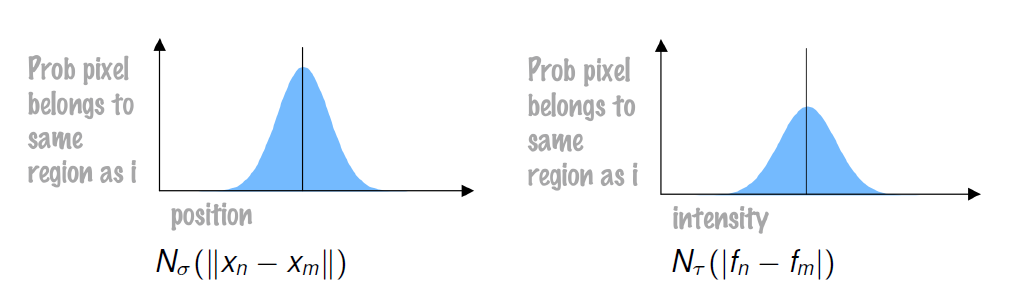
\includegraphics[width=\textwidth]{images/chap1/bilateral}, $x_n,x_m$ being pixel positions and $f_n, f_m$ pixel intensities, $\sigma, \tau$ the standard deviation for the two gaussian dists. $N_\sigma, N_\tau$. The filter in $n$-th pixel is defined as: $$g(n) = \dfrac{1}{K_n} \sum\limits_{m=1}^N f_m N_\sigma(||x_n - x_m||) N_\tau (|f_n -f_m|)$$ with $$K_n = \sum\limits_{m=1}^N N_\sigma(||x_n - x_m||) N_\tau (|f_n -f_m|)$$.

Sum is defined over all pixels, usually only small window of size $3\sigma$ around $x_n$ is used. $\tau \rightarrow \infty$ approx. gaussian filter.

\subsection{Non-local means}

\textbf{Idea:} Images have similar patches over the image, average using most similar patches. Formally: For each pixen $n$, define $k\times k$ window of pixels $W_n$, vector of pixel indices. Distance $d_{n,m}$ defined as $$d^2_{n,m} = \sum\limits_{s=1}^{k^2} (f(W_n(s)) - f(W_m(s)))^2$$ and kernel weights $$k_{n,m} = e^{-\frac{d_{n,m}^2}{2\sigma^2}}$$, the $n$-th pixel then is deifined as $$g(n) = \dfrac{1}{\sum\limits_{m=1}^{N} k_{n,m}} \sum\limits_{m=1}^N k_{n,m} f_m$$,

usually also restricted to a window. \textbf{Very expensive and slow}.

\subsection{Denoising Salt and Pepper Noise}

Average filter gives bad result. Use \textbf{Median Filter}! High-valued and low-valued outliers won't have a strong effect on the result this way.
























\chapter{Detecting Features and Patterns}

\section{Image edges and image derivatives}

\textbf{Goal:} Identify sudden changes in an image. Most semantic shape information is within edges.

\textbf{Causes for edges:} Reflection changes (appearance information and texture), Depth discontinuity, Shadows, Changes in surface orientation (shape).

Plotted using itensity as height, edges appear as "cliffs" $\rightarrow$ Low-level edges characterized by \textbf{gradient magnitude}.

\textbf{Problems of edge detection:} Intensity changes are often not linked to the actual object contours, hence we get a lot of unuseful information. Causes can be: Strong intensity changes (texture, shadows), No intensity change at boundary (background texture similar, too dark,...).

Human edge detection: High-level (object-level), completion of invisible contours, shadow removal, ... .

\textbf{Concentrating on gradient-based edge detection}!

\subsection{Image derivatives}

\textbf{Continuous derivative:} $\partial_x f(x,y) = \lim_{\epsilon \rightarrow \infty} \dfrac{f(x + \epsilon, y) -f(x,y)}{\epsilon}$

\textbf{Discrete versions:}

\begin{description}
    \item[Forward diff.] $(\partial_x f)_{i,j}) = \dfrac{f(i+1,j) - f(i,j)}{h_x}$
    \item[Backward diff.] $(\partial_x f)_{i,j}) = \dfrac{f(i,j) - f(i-1,j)}{h_x}$
    \item[Central diff.] $(\partial_x f)_{i,j}) = \dfrac{f(i+1,j) - f(i-1,j)}{2h_x}$
\end{description}

With (convolution) kernels $[1,-1,0], [0,1,-1], [1/2, 0, -1/2]$. The same holds for derivative in y-direction, only with transposed vectors, i.e., column vector.

\textbf{Gradient:} The gradient $\nabla f = (\partial_x f, \partial_y f)$ is the derivative in both directions and can be interpreted as vector-valued image with $n=m=2$, the gradient points strongest changes in each direction.

\textbf{Gradient magnitude:} $||\nabla f|| = \sqrt{(\partial_x f)^2 + (\partial_y f)^2}$ is the length of the vector. \textbf{Larger magnitude, stronger changes}.

Problems with noise and derivatives:\textbf{ High frequency content is amplified, since they are strong changes!} Hence, first smooth signal (image) then apply derivative.

\subsection{Convolution and Derivatives}

Smoothing needs convolving, which is needed when noisy image derivatives are to be calculated.

\textbf{Continuous Conv.:} $(f*g)(x) = \int_{\mathbb{R}^N} f(x-u)g(u) du$, same as discrete only with integral.

\textbf{Derivative theorem for cont. conv.:} $\partial_i (f*g) = (\partial_i f)*g = f * (\partial_i g)$, more efficient to only have to calculate one derivative. Needs some conditions on $f$ and $g$!

When met, a kernel derivative can be precomputed and applied using convolution (for instance Gaussian on LS 2.20).

\textbf{Advantages:} Precomputation (Efficiency); Filter function is known, then coefficients can be precomuted analytically!

\textbf{Example:} Derivative using gaussian derivative filter: 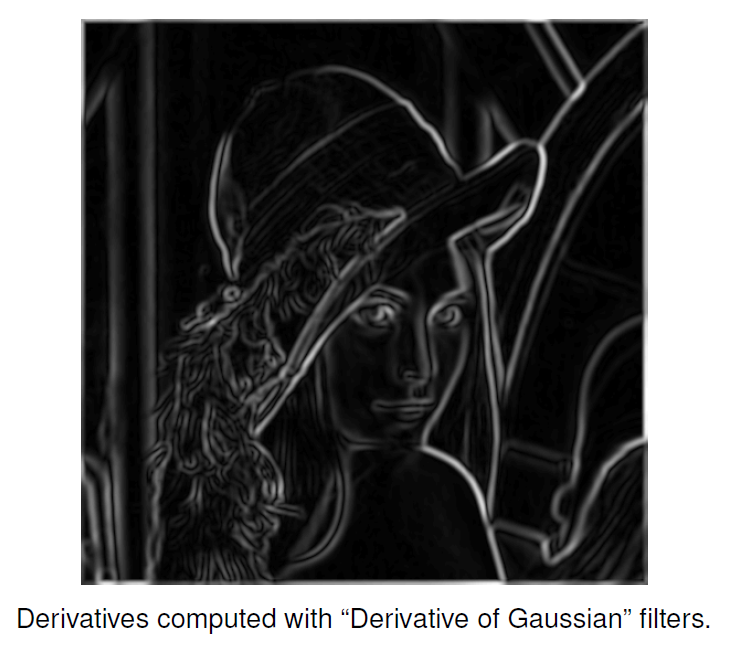
\includegraphics[width=.3\textwidth]{images/chap3/der_gauss}

\subsection{Canny Edge Detection}

How to find the edge when we have the derivative image?

\textbf{Non-maxima suppression idea:} Keep pixels that are on local maxima along the gradient direction (interpolation).

\textbf{Process:}

\begin{itemize}
    \item Filter with derivative of gaussian at scale $\sigma$
    \item Find magnitude and oritentation of gradient
    \item Non-maxima suppression!
    \item Linking, thresholding, two thresholds \textbf{low and max}, low starts edges and high continues them.
\end{itemize}

\subsection{Scale-space}

Applying gaussian filter with incrementing $\sigma$ removes "detail": \textbf{Scale-space}

\begin{itemize}
    \item Edges may shift with increasing $\sigma$
    \item Edges may merge!
    \item Edges may not split into two
    \item Multiple ways to calculate scale-spaces, \textbf{gaussian} is the "canonical" one
\end{itemize}

\section{Feature detection: the fundamentals}

\textbf{Steps for matching:}

\begin{itemize}
    \item \textbf{Detection}, identify points
    \item \textbf{Description}, extract information (feature vector)
    \item \textbf{Match}, correspondences between descriptors
\end{itemize}

\textbf{Goals for detectors:}

\begin{itemize}
    \item \textbf{Locality}, features local, robust to occlusion and clutter
    \item \textbf{Quantity}, many for one image
    \item \textbf{Distinctiveness}, differentiate large amount of objects
    \item \textbf{Efficiency}, real-time scalability
    \item \textbf{Geometric invariance}, translation, rotation, scale!!
    \item \textbf{Photometric invariance}, intensity, brighteness, contrast, exposure
\end{itemize}

\subsection{Good features}
\textbf{What points to choose?}: Large contrast changes, gradients in two different image orientations (corners)..

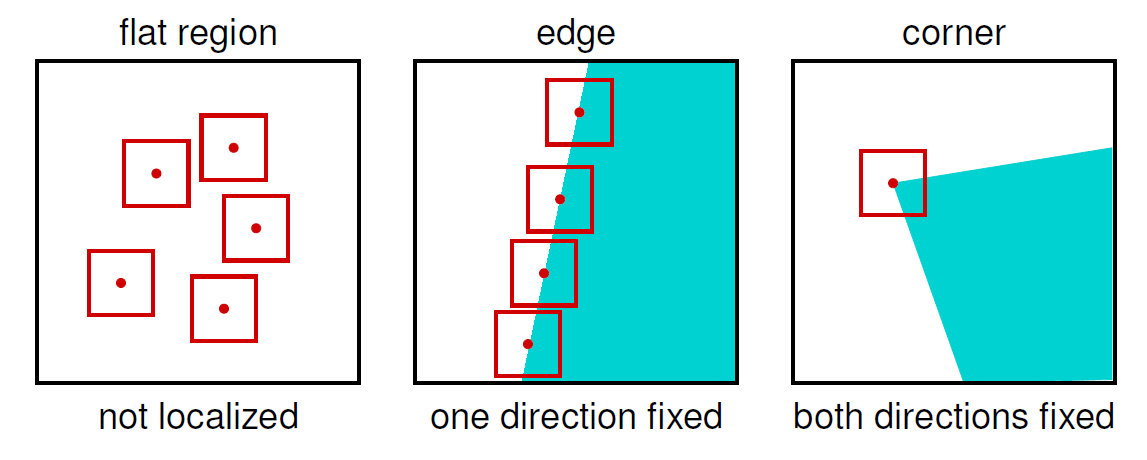
\includegraphics[width=.7\textwidth]{images/chap3/good_feature}

The image shows that only corners have unique regions, even on edges we have multiple similar patches.

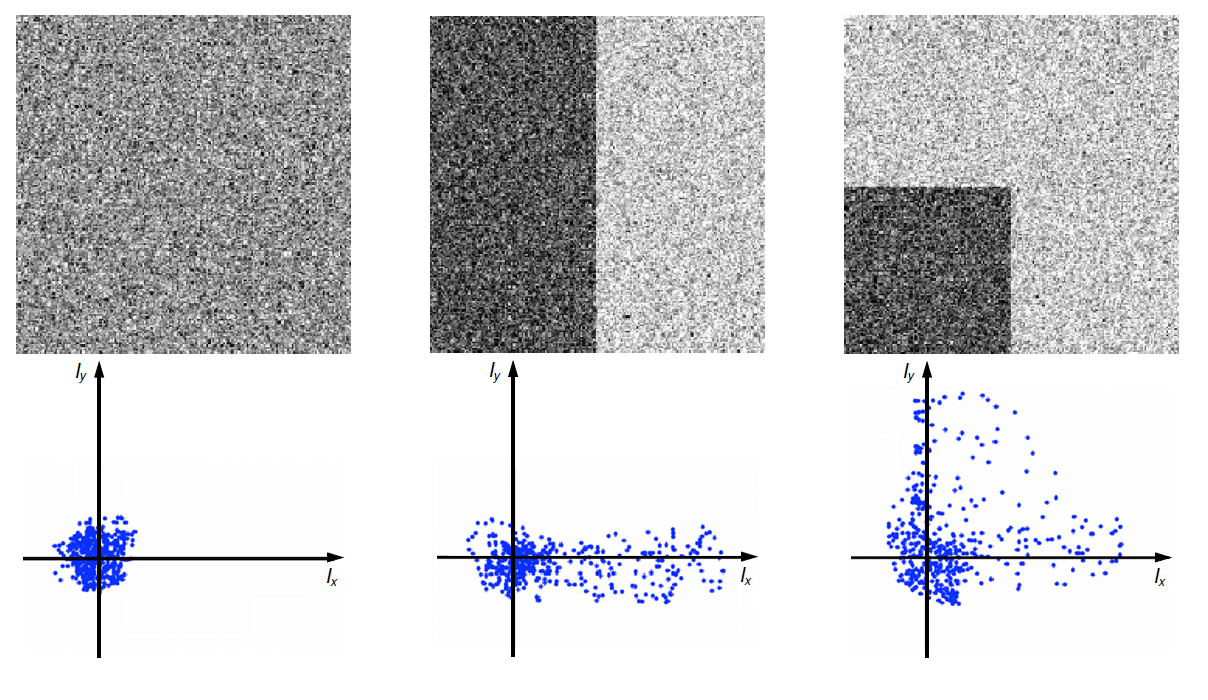
\includegraphics[width=.7\textwidth]{images/chap3/feature_dist}

This image shows the distribution of data. When we have a corner, we have points in both directions.

\subsection{Maths: SVD}

A matrix $A \in \mathbb{R}^{m\times n}$ can be factorized in the form of $A = U \Sigma V^T$, where

\begin{itemize}
    \item $U \in \mathbb{R}^{m\times m}$ is orthogonal, $UU^T = U^T U = I_m$
    \item $V \in \mathbb{R}^{n \times n}$ is orthogonal 
    \item $\Sigma \in \mathbb{R}^{m\times n}$ is diagonal, sorted non-neg. real numbers $\sigma_1 \geq \sigma_2 \geq ... \geq 0$ and are called singular values of A.
\end{itemize}

\textbf{Singular values} are uniquely determined, $U,V$ are not. $AV = \Sigma U$ shows that, $A$ maps $V$ to $U$ scaled by $\Sigma$.
\begin{itemize}
\item \textbf{Rank of matrix:} Number of non-zero singular values
\item \textbf{Range of $A$:} Spanned by columns of $U$ where singular values non-zero (i.e. rank)
\item Columns of $V$ are eigenvectors of $A^T A$
\item Columns of $U$ are eigenvectors of $AA^T$
\item Eigenvalues of $A^T A$ and $AA^T$ are squared singular values.
\item Eigenvalues only positive or zero.
\end{itemize}

\textbf{Applications:}

\begin{itemize}
    \item Can solve problems of type $argmin_{|x| = 1} ||A_x||$
    \item PCA
    \item Linear least square for homography estimation  $argmin_{|x| = 1} ||A_x - b||^2$
\end{itemize}

\textbf{Interpretation:}

\begin{itemize}
    \item Columns of $V$ give new basis for vector space $\mathbb{R}^n$
    \item Face data: Space of possible images of faces
    \item New basis vectors are chosen to capture most important aspects of data in descending order of importance
    \item Importance corresponds to magnitude of singular value
\end{itemize}

\textbf{PCA:} Intuition of SVD is formalized in PCA. Goal is to characterize probability dists. of variables, for example to find the directions with greatest variance.

\textbf{Joint probability distributions terminology}:

\begin{itemize}
    \item Random Variables $X_j, j=1,..,n$, two variables we call it \textbf{bivariate}
    \item \textbf{Joint distribution}, $P(X_j=x_j \forall j)$ in the image, samples inside green ellipse
    \item Marginal distributions, $P(X_j = x_j)$, i.e., $P(X=x)(blue), P(Y=y)(red)$ in the image.
    \item $X_j, X_k$ independent iff  $P(X_j=x_j, X_k=x_k) = P(X_j = x_j)P(X_k=x_k)$
\end{itemize}

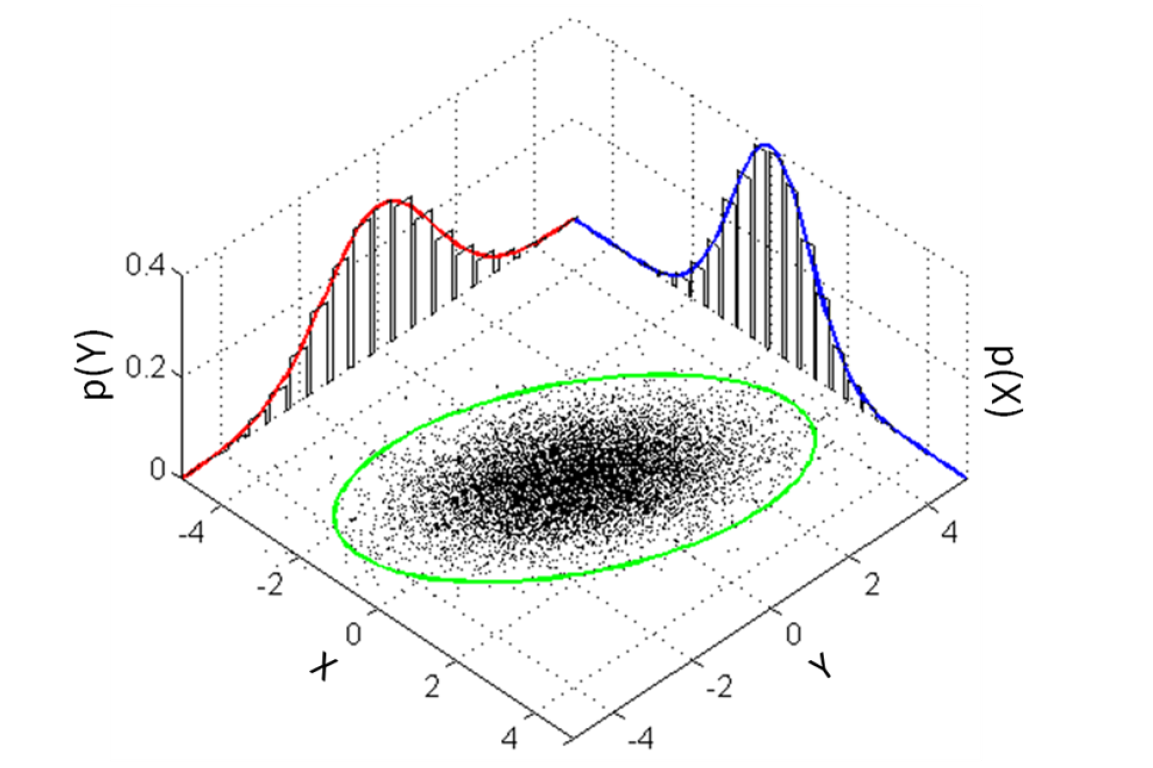
\includegraphics[width=.7\textwidth]{images/chap3/joint_dist}

\textbf{Expected sample value:}  $E(Z) = \sum p_iz_i$, weighted average over all measurements for $Z$.

\textbf{Sample variance:} $Var(Z) = \sum p_i(Z_i - E(Z))^2$, expected squared deviation from the expectation value.

\textbf{Sample standard deviation:} Squareroot of variance is $\sigma(Z)$

\textbf{Covariance of two random Variables X,Y:} $cov(X,Y) = \sum p_i(x_i - E(X))(y_i - E(Y))$.

\textit{Assuming we have centered measurements}, i.e. $E(Z_i) = 0$ for all $Z_i$. Then the covariance is $cov(X_j,X_k) = \sum p_i x_{ji} x_{ki}$.

\textbf{Covariance matrix:} Defined as $n\times n$ matrix for $n$ random variables:

$C(X) := (cov(X_j,X_k))_{j,k=1,\dots,n}$ and properties are: \textbf{Symmetric, Diagonal is Variances, positive semi-definite}. If measurements are row vectors of large matrix $M \in \mathbb{R}^{m\times n}$ and i-th row is multiplied by $\sqrt{p_i}$, we have $C(X) = M^T M$.

\textbf{Covariance Matrix and SVD}

If $M = U \Sigma V^T$, measurements transformed by $V$, we get $M' = MV = U\Sigma$ with cov. $C' = \Sigma^T U^T U \Sigma = \Sigma^2$, i.e., cov. matrix can be made diagonal using orthogonal tranformation! (Eigenvectors of old cov. matrix are mapped to unit vectors). The standard deviations are equal to the singular values.

\textbf{Ellipses}: Two random variables decorrelated. Ellipse given as: 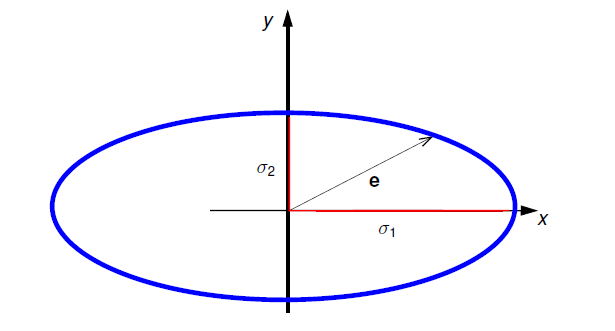
\includegraphics[width=.3\textwidth]{images/chap3/ellipse}

\textbf{Interpretation:} Radius $e = (\sin(\Phi),\cos(\Phi))^T$ is $\sqrt{\sigma_1^2e_1^2+\sigma_2^2e_2^2} = \sqrt{e_1^2 var(X) + e_2^2 var(Y)} = \sqrt{var(e_1X+e_2Y)}$, i.e., radius yields standard deviation projected onto the direction (denoted by $\Phi$).

\textbf{Summary of PCA}

\begin{itemize}
    \item Closely related to SVD
    \item Use to decorrelate data
    \item Dimensions with larger singular values have higher variance, more meaningful
    \item Useful for high-dimensional data analysis, find most meaninungful lower-dimensional representation
    \item Application for gradient measurements around a pixel to analyze local orientations in images
\end{itemize}

\subsection{Structure Tensor}

Gaussian kernel $G_\sigma$, derivative is with scale $\sigma$ is $\partial_x^\sigma = \partial_x * G_\sigma$, for images $f = (f_{i,j})$ we write the partial der. at scale $\sigma$ as $f_x^\sigma, f_y^\sigma$.

\textbf{ST as gradient statistics:} Sample gradient scale $\sigma$ of window for pixel. Interested in local structure, assign weight depending on distance to pixel (gaussian distribution).

Consider gradient to be distributed as \textbf{joint distribution} of partial derivatives $f_x^\sigma, f_y^\sigma$. The distribution around the pixel (i,j) is characterized by the cov. matrix:

$$C(\nabla^\sigma f) = \left[
\begin{matrix}
cov(f_x^\sigma , f_x^\sigma) & cov(f_x^\sigma , f_y^\sigma) \\
cov(f_y^\sigma , f_x^\sigma) & cov(f_y^\sigma , f_y^\sigma)
\end{matrix}\right] = \left[
\begin{matrix}
E(f_x^\sigma f_x^\sigma) & E(f_x^\sigma f_y^\sigma) \\
E(f_y^\sigma f_x^\sigma) & E(f_y^\sigma f_y^\sigma)
\end{matrix}\right]$$

Expanding the formulas, gives the definition of the !\textbf{structure tensor}!, which is
$$\tau = \left[
\begin{matrix}
G_\tau * (f_x^\sigma)^2 & G_\tau * (f_x^\sigma f_y^\sigma) \\
G_\tau * (f_x^\sigma f_y^\sigma) & G_\tau * (f_y^\sigma)^2
\end{matrix}\right] = G_\tau * \left[
\begin{matrix}
 (f_x^\sigma)^2 & (f_x^\sigma f_y^\sigma) \\
(f_x^\sigma f_y^\sigma) & (f_y^\sigma)^2
\end{matrix}\right]$$

a grayscale image whose values are $2\times 2$ matrices. Two parameters are necessary, $\sigma > 0$ is the inner scale for the derivatives and $\tau > 0$ the outer scale parameter which determines the size of the window on which the derivative information is sampled on. Example: \\
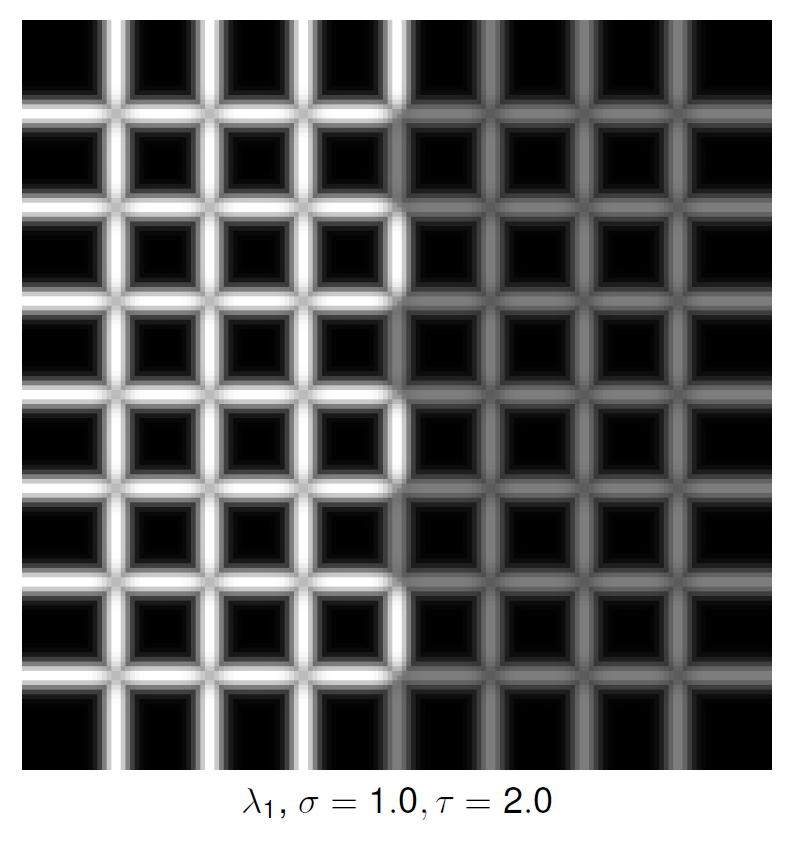
\includegraphics[width=.5\textwidth]{images/chap3/st_ex}

for a checkerboard image and $\lambda_1$ being the first eigenvalue (biggest as well). For $\lambda_2$ boxes can be seen in the example on LS 2.74.

\textbf{Properties based on eigenvalues:}

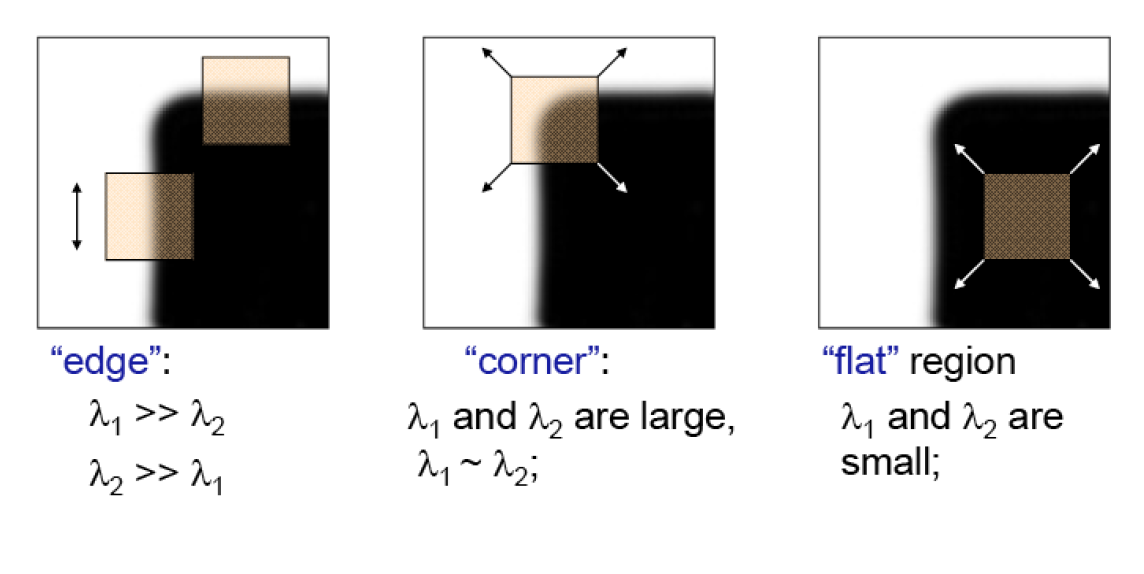
\includegraphics[width=.6\textwidth]{images/chap3/st_props}, i.e. edges are denoted s.t. one of the eigenvalues is much larger, for corners both are large and flat regions both are small. 

\textbf{Cornerness response function:} $\lambda_1 \geq \lambda_2$, multiple functions exist to tell if a point looks like a corner: 

\begin{itemize}
    \item Shi and Tomasi, 1994: $\lambda_2$ smaller is used
    \item Harrise 1988, Foerstner 1986: using $\det(\tau) - \mathcal{K} trace(\tau)^2 = \lambda_1 \lambda_2 - \mathcal{K}(\lambda_1+\lambda_2)^2$
\end{itemize}

Corners are found when a threshold is exceeded and a local maximum is reached.

\section{Pattern matching}

\textbf{Patch comparison:} SSD - sum of squared diffs.: $$E_{SSD}(f,g) = \sum_i^W\sum_j^H (f(i,j)-g(i,j))^2$$, W being the width and H the height of the patch. Example of paramentrization:

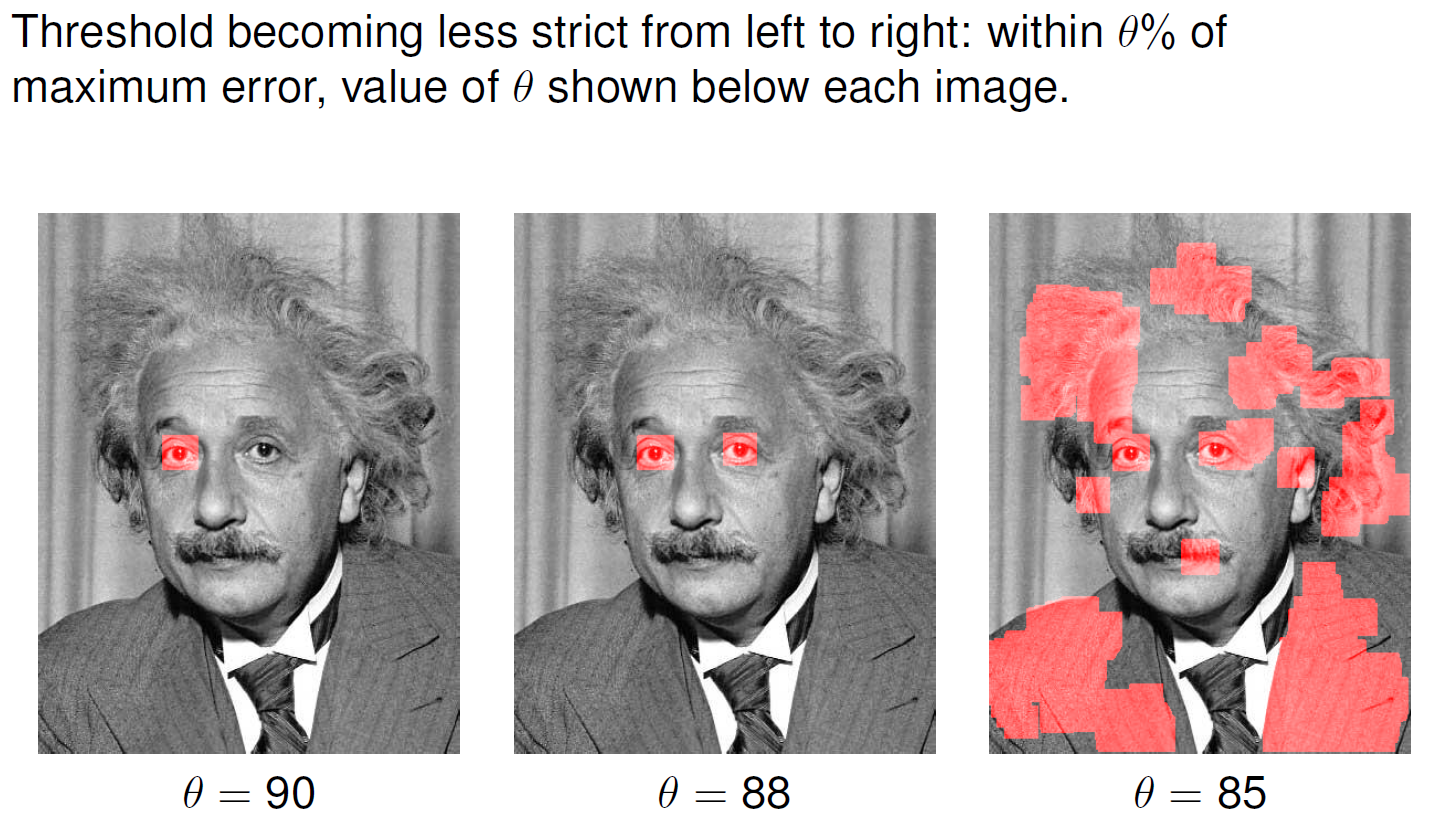
\includegraphics[width=.6\textwidth]{images/chap3/SSD_thresh}

\textbf{Properties as patch comparison metric:}
\begin{tabular}{lr}
    Fast & yes \\
    \hline    
    Invariant to translation & yes \\
    Invariant to rotation & no \\
    Invariant to scaling & no \\
    \hline
    invariant to contrast/brightness changes & No
\end{tabular}

\textbf{Better approach? NCC!}: Given a patch W,H on f,g the \textbf{Normalized Cross-Correlation} distance is defined as $$E_{NCC}(f,g) = \dfrac{cov(f,g)}{\sigma(f)\sigma(g)}$$, range within [-1,1], larger the better.

\textbf{Properties as patch comparison metric:}
\begin{tabular}{lr}
    Fast & no \\
    \hline    
    Invariant to translation & yes \\
    Invariant to rotation & no \\
    Invariant to scaling & no \\
    \hline
    invariant to contrast/brightness changes & yes
\end{tabular}

\textbf{Autocorrelation:} Idea is to displace patch location slightly by a shift vector $u$, check old with new using \textbf{weighted} SSD. This approach gives an idea of the stability of the patch. \textbf{Definition:}

Weight $w(p_i)$ in each pixel, for instance gaussian dist. $\tau$ around patch center. Autocorrelation for patch $f$ shift $u$ weight $w$ is defined as weighted SSD: $$E_{AC} (f,u) = \sum_i w(p_i)(f(p_i+u)-f(p_i))^2$$, sum running over all pixels.

\textbf{Intuition:} AC small if patch shifted s.t. it looks similar.

\textbf{AC approximation for small $u$:} Step 1: Taylor series approximation of $f$ around each pixel $$f(p_i + u) \approx f(p_i) + \nabla f(p_i)^T \cdot u$$, i.e. add the gradient multiplied by the shift vector to the original.

Step 2: Compute $E_{AC}$ using following approximation (sum of weights applied to difference of taylor series approximations from the pixels all pixels), which eventually results in the following equation $$E_{AC}(f,u) \approx u^T \left(\sum_i w(p_i) \nabla f(p_i) \nabla f(p_i)^T\right) u$$ the middle part $\left(\sum_i w(p_i) \nabla f(p_i) \nabla f(p_i)^T\right)$ being the structure tensor again! Two interpretations for the ST now: I.e., \textbf{1.} the structure tensor being the cov. matrix of the gradient distribution and \textbf{2}. $$E_{AC} = u^T \tau u$$ as an approx. for the AC for small shifts.

\textbf{Autocorrelation maxima/minima:} Find direction of fastest increase of error, i.e., $||u|| = $ s.t. $u^T \tau u $ is maximal. With eigenvalue decomp. of $\tau$, $\lambda_1 \geq \lambda_2$ we get :

$$u^T \tau u = (u^T V) \left[\begin{matrix} \lambda_1 & 0 \\ 0 & \lambda_2 \end{matrix}\right] (V^T u)$$

\subsection{Summaries}

\textbf{Edges:} \begin{itemize}
    \item Edges are of interest, since they denote fast changes in images
    \item Edges as locations of strong image gradients
    \item Gradient computed at different image scales (using gaussian pre filtering) - noise removal and selecting dominant edges when moving towards larger scales
    \item Popular edge-detector \textbf{Canny}, combining non-max. suppression and thresholding to follow contours
\end{itemize}

\textbf{Corners:} \begin{itemize}
    \item Edges "one" direction, Corners "two" and patches are uniquely identified by corners
    \item Characterized by distribution of gradient - strong gradient in two orthogonal directions
    \item ST as cov. matrix of gradient distribution is used to detect corners, eigenvalues give edge strength in eigenvector direction
    \item Alternative interpretation: ST is approx. of autocorrelation, EVectors and EVals describe rate of change when patch is shifted
\end{itemize}

\textbf{Pattern Matching:} \begin{itemize}
    \item SSD used for comparing patches
    \item Not robust against brightness and contrast changes
    \item NCC  is robust against those
    \item SSD is faster than NCC
\end{itemize}






















\chapter{Frequency and Scale}

\section{Thinking in Frequency: Fourier Transform}
\subsection{Hybrid images}
How does it work? Take low freq. content from one image and high freq content from another. On long distance humans can see only low frequency content.

\textbf{Fouriers idea}: Any univariate function can be rewritten as a weighted sum of sines and cosines of different frequencies.

\subsection{Waves in 2D} A 2D wave for an image is given as $f(x,y) = r \cos(2\pi (\omega_x x + \omega_y y) + \phi)$, $\omega = [\omega_x \omega_y]$ being the \textbf{wave number}, $f = |\omega|_2$ the frequency, $\omega /f$ the direction of the wave and $\phi$ the phase, $r$ the amplitude. 

Examples are given by

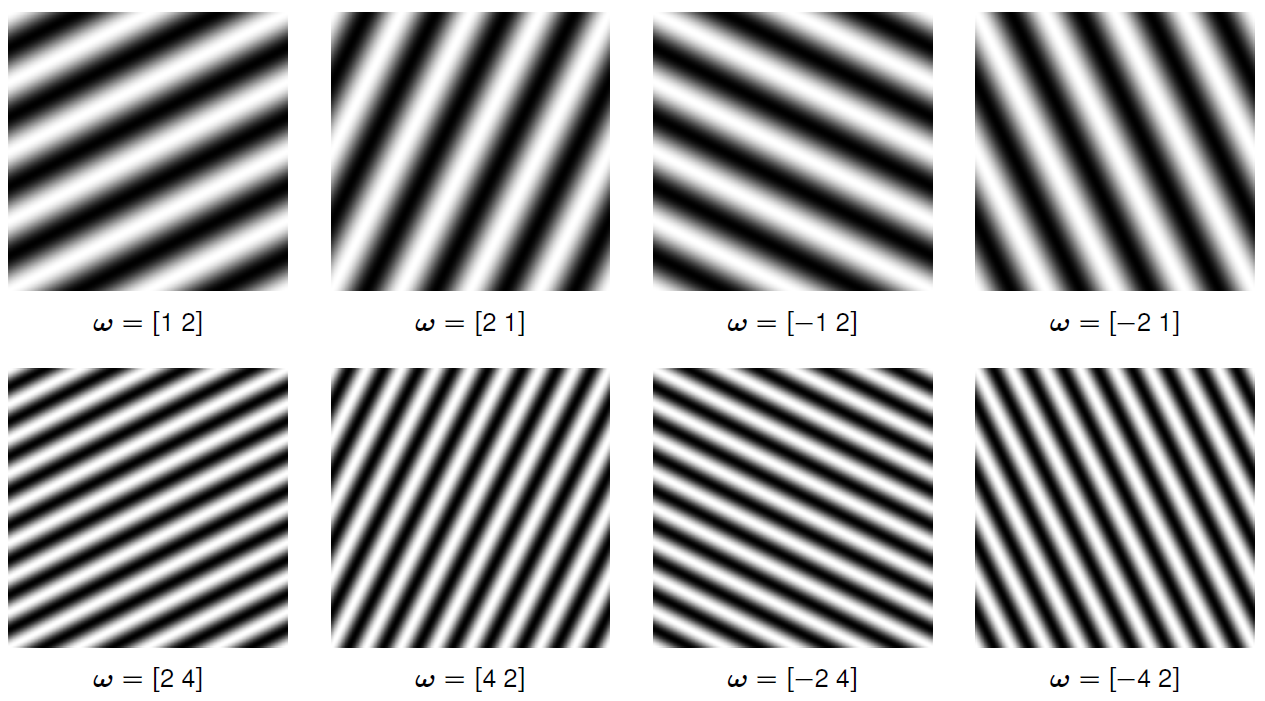
\includegraphics[width=.7\textwidth]{images/chap4/freq_examples}, varying the phase, shifts the signals position.

\textbf{Complex elementary wave}: For $\omega = [\omega_x \omega_y]$, $W_\omega (p) = e^{2\pi i (\omega p)} = \cos(2\pi(\omega p)) + i \sin(2\pi (\omega p))$, with phase zero, amp. one.

\textbf{Central idea of fourier transform:}

\begin{align*}
    f(p) & = \int_{\mathbb{R}^2} \hat{f}(\omega) W_\omega (p) d\omega \\
    & = \int_{\mathbb{R}}\int_{\mathbb{R}} \hat{f} (\omega_x, \omega_y) e^{2\pi i(\omega_x x + \omega_y y)} d\omega_x d\omega_y
\end{align*}, $\hat{f}$ being the fourier transform of $f$.

\textbf{Observations:}

\begin{itemize}
    \item Sum of signals, is sum of fourier transforms
    \item Getting rid of imag. part in a complex wave, is adding it with it's conjugate
    \item Noise amplifies large frequencies
    \item Cutting out a section of the fourier transform is similar to blurring (Low-pass)
    \item Phase is more important for how a picture looks like
\end{itemize}

\textbf{Inner product of complex numbers z,w:} Multiply $z$ b y comp. conjugate of $w$! (Hermitian inner product).

\textbf{Inner product for function $f,g: \mathbb{R}^2 \rightarrow \mathbb{C}$}: $(f,g)_{\mathbb{C}}$ is a function as a vector with infinitely many components. Summing over components becomes an integral and we get 
\begin{align*}
    (f,g)_{\mathbb{C}} & = \int_{\mathbb{R}^2} f(p) \overline{g}(p) dp \\
    & = \int_{\mathbb{R}}\int_{\mathbb{R}} f(x,y) \overline{g}(x,y) dx dy
\end{align*}

The \textbf{fourier coefficients} are then defined as:
\begin{align*}
    \hat{f}(\omega) & = (f,W_\omega)_{\mathbb{C}}\\
    & = \int_{\mathbb{R}^2} f(p) \overline{W}_\omega(p) dp \\
    & = \int_{\mathbb{R}}\int_{\mathbb{R}} f(x,y) e^{-2\pi i(\omega_x x + \omega_y y)} dx dy
\end{align*}

\section{Filtering in frequency space}

\subsection{Shifting theorem and convolution theorem}

Shifting a wave by vector $p_0$ results in a phase shift by $2\pi \omega \cdot p_0$,i.e., $e^{2\pi i \omega p} e^{-2\pi i \omega p_0} = e^{2\pi i \omega (p-p_0)}$. For the \textbf{FT} this means shifting by a vector $p_0$ means shifting all elementary waves by $e^{-2\pi i \omega \cdot p_0}$.

\textbf{Convolution:} Is the same as multipliying the corresponding elementary waves one by one. Hence $\hat{f * g} = \hat{f} \hat{g}$.

The \textbf{FT} of a gaussian is a gaussian-like function. When looking at the image, one can see that it corresponds to a low-pass filter.

\begin{itemize}
    \item Low-pass: gaussian
    \item High-pass: Impulse minus gaussian
    \item Band-pass: Difference of gaussians
\end{itemize}

\subsection{Derivatives and the fourier transform}

Taking derivatives amplifies high frequencies, higher frequency and derivative order, higher amplification.

\begin{align*}
    \partial_x^n\partial_y^m f(p) & = \int_{\mathbb{R}}\int_{\mathbb{R}} \hat{f}(\omega) \partial_x^n\partial_y^m[e^{2\pi i(\omega_x x + \omega_y y)}] dx dy \\
    & = \int_{\mathbb{R}^2} (2\pi i \omega_x)^n (2\pi i \omega_y)^m \hat{f}(\omega) W_\omega (p) dp \\
 \hat{\partial_x^n\partial_y^m} f(\omega) & = (2\pi i \omega_x)^n (2\pi i \omega_y)^m \hat{f}(\omega)
\end{align*}

\textbf{Properties of the FT:}

\begin{itemize}
    \item Linearity: Constant factor and additive
    \item Rotation invariant: Rotation of $f$ means rotation of $\hat{f}$ (same angle)
    \item Shift theorem
    \item Convolution theorem
    \item Derivatives
\end{itemize}

\section{Sampling and image pyramids}

\subsection{Sampling and aliasing}

Remember, naively finding a patch is not scale invariant. If the image has too many pixels compared to a patch we need to downsample the image, since both patch and image resolution have to be the same.

\textbf{Sampling theorem:} $f$ band-limited, i.e., highest frequency $W$ exists with $\hat{f} (\omega) = 0 if |\omega|_2 > W$. The sampling rate has to be twice as high.

For sampling distance $h$ this means $h < h_{max} = 1/2W$.

\textbf{Downsampling:} Depending on the highest frequency in the image, at a certain point we get aliasing. Downsampling means reducing sampling distance $h$, reducing nyquist frequency as well.

\textbf{Solution:} Band-limit signal further before down sampling.

\subsection{Gaussian pyramids}

Gaussian prefiltering: blur $\rightarrow$ downsample $\rightarrow$ blur $\rightarrow \dots$.

\textbf{Gaussian pyramid:} Represent $N\times N$ image as subimages of powers of 2 resulting in a pyramid:

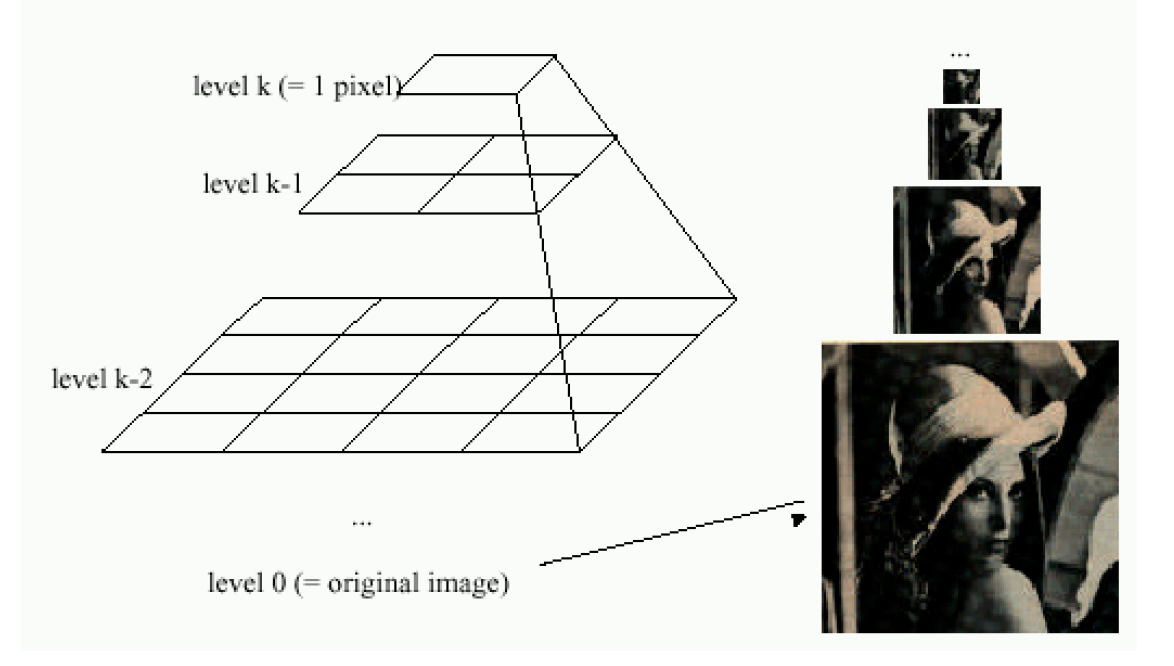
\includegraphics[width=.7\textwidth]{images/chap4/gaus_pyra}

For this we have approx. $4/3$ storage space requirement.

\subsection{Laplacian pyramids}

Different idea: Instead of storing the full image at subsequent levels, we store the high-frequency content, i.e. the difference of gaussians at each level.

\section{Summary}

\textbf{FT:}

\begin{itemize}
    \item CFT analyzes frequency content of images
    \item Decomposition into superposition of elementary waves
    \item Complex fourier coeffs. represent amplitude and phase
    \item Linear, Invariant under rotations
    \item Spatial shifts are phase shifts
    \item Differentiation becomes multiplication with the frequency
    \item Convolution becomes point-wise multiplication
    \item Highly useful for analyzing frequency behavior of conv. filters
\end{itemize}

\textbf{Aliasing, subsampling:}

\begin{itemize}
    \item Sampling at twice the nyquist rate
    \item Filtering before downsampling
    \item Continued downsampling leads to pyramids, representations at different scales
    \item Gaussian is low pass filter, Laplacian a bandpass decomposition
    \item Both redundant, need more disk space
\end{itemize}




























\chapter{SIFT}

\section{Introduction}

\subsection{Distinctive Image Features from Scale-Invariant Keypoints}

\textbf{Goals:} \begin{itemize}
    \item Detect features in images (mainly corners)
    \item Detailed descriptor, as unique as possible
    \item Invariance in location, scale and orientation
\end{itemize}

\textbf{Applications:} \begin{itemize}
    \item Find sparse correspondences between images
    \item Estimate global rotations (stereo geometry, homographies, parametric transformations)
    \item Tracking, Structure from Motion
    \item Object detection, recognition
\end{itemize}

\subsection{The Scale-Invariant Feature Transform}

\textbf{Step 1:} Detect characteristic feature points.

\textit{Based on Gauss. scale-space using DoG; Extrema provide location and scale}

\textbf{Step 2:} Accurate localisation of key points

\textit{Subpixel refinement fitting quadratic functions; Discard points with high ration between principal curvatures}

\textbf{Step 3:} Assignment of dominant orientations

\textit{Histogram of gradients in local neighborhood; Refines orientation, fitting quadratic functions.}

\textbf{Step 4:} Computation of a suitable key point descriptor

\textit{Unit vector based on accumulated histograms of gradients; compensated by location, scale and dominant orientation}

\textbf{Remark:} Steps not difficult, lots of engineering needed for max. quality.

\section{SIFT feature detection}

\subsection{Step 1: Detection of characteristic feature points}

\subsubsection{Detection of scale-space extrema}

\textbf{Starting point: Gaussian Scale-Space of input image $f$}

Using discrete levels of smoothing again, i.e., $\sigma_0, \sigma_1, \dots$. Consecutive levels related by: $\sigma_{t+1} = k_{\sigma_t}, k > 1$. 

Scale-space is given by convolution of $f$ with increasing gaussian $f_t = G_{\sigma_t} * f$. 

\textbf{From this: DoG}

Difference of two consecutive scales: \begin{align*}
    D_t & = f_{t+1} - f_t \\
    & = G_{k\sigma_t} * f - G_{\sigma_t} * f \\
    & = (G_{k\sigma_t} - G_{\sigma_t}) * f
\end{align*}

DoG is bandpass filter, only details of a scale level survive.

\textbf{Idea:} Feature is strongest detector response in a scale, search for max. across scales for \textbf{scale invariance}.

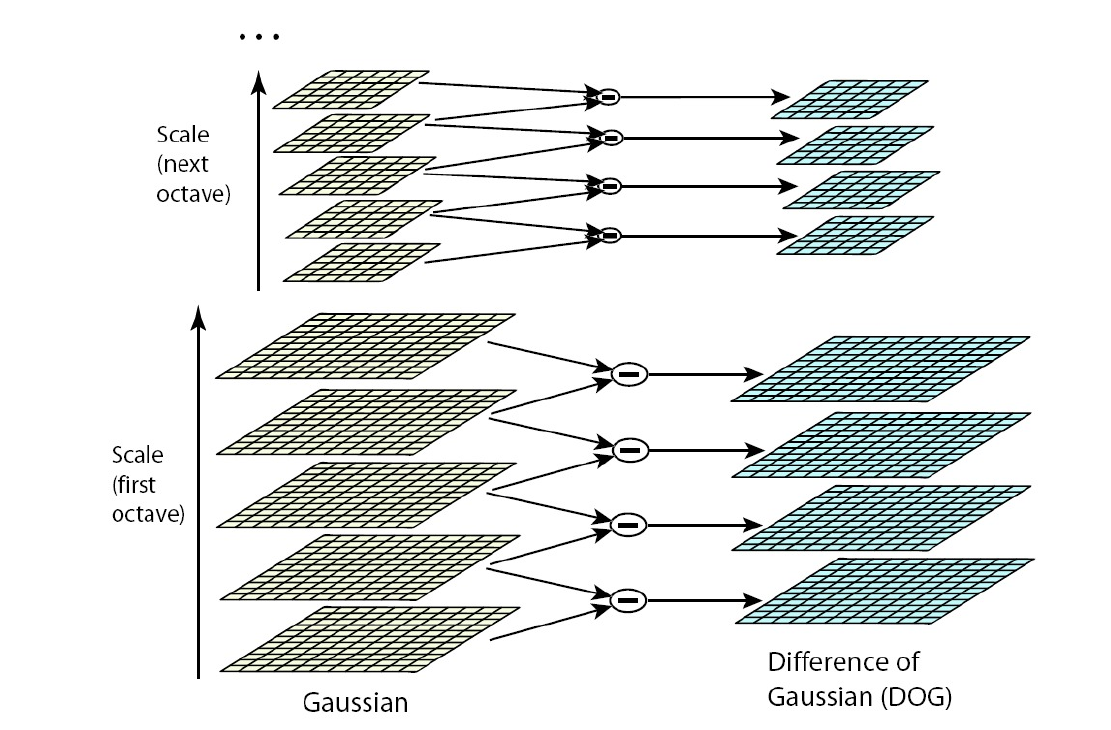
\includegraphics[width=\textwidth]{images/chap5/sift_DOG}

Here resolution is halved every octave. Original impl. uses $\sigma_0 = 0.5$ and $\rho = \sqrt{2}$.

\textbf{DoG and Laplacian-of-Gaussian}: \textit{DoG} related to scale derivative of Gaussian with following approx: $\partial_\sigma G_\sigma \approx \dfrac{G_{k\sigma} - G_\sigma}{k\sigma - \sigma}$ and the analytic derivative is the \textbf{Laplacian of Gaussian (LoG):} $$\partial_\sigma G_\sigma = \sigma \Delta G_\sigma = \sigma(\partial^2_x G_\sigma + \partial^2_y G_\sigma)$$

\textbf{Result:} DoG is approx. of scaled \textbf{LoG} with constant factor: $$G_{k\sigma} - G_\sigma \approx (k-1)\sigma^2 \Delta G_\sigma$$, but $(k-1)$ can be neglected, no influence on locations of extremal positions! $\sigma^2 \Delta G_\sigma$ is called \textbf{normalized Laplacian-of-Gaussian}! (This is also equivalence of scale space construction to heat diffusion!)

\textbf{Detection:} Filters "detect" shapes similar to their own, i.e., the LoG finds \textbf{BLOBS}. Following pictures depict scale-space for LoG:

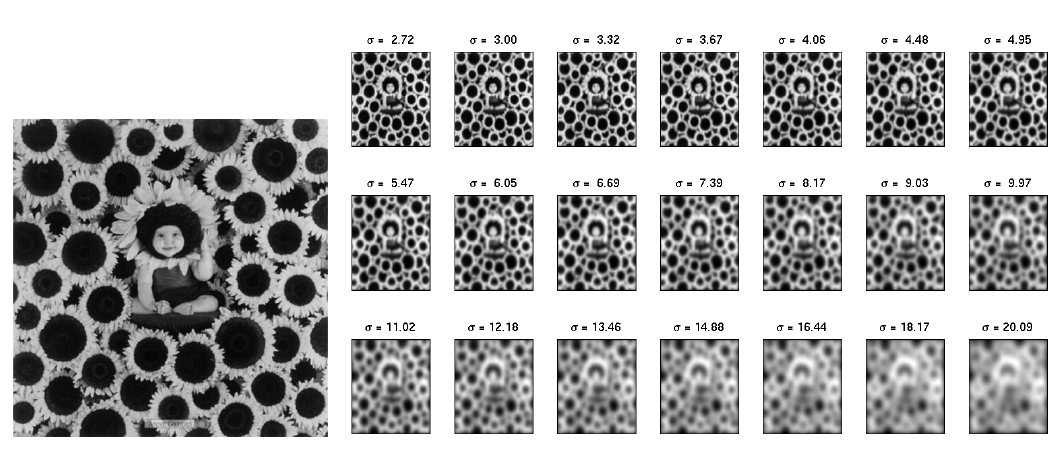
\includegraphics[width=\textwidth]{images/chap5/LOG}

and normalized

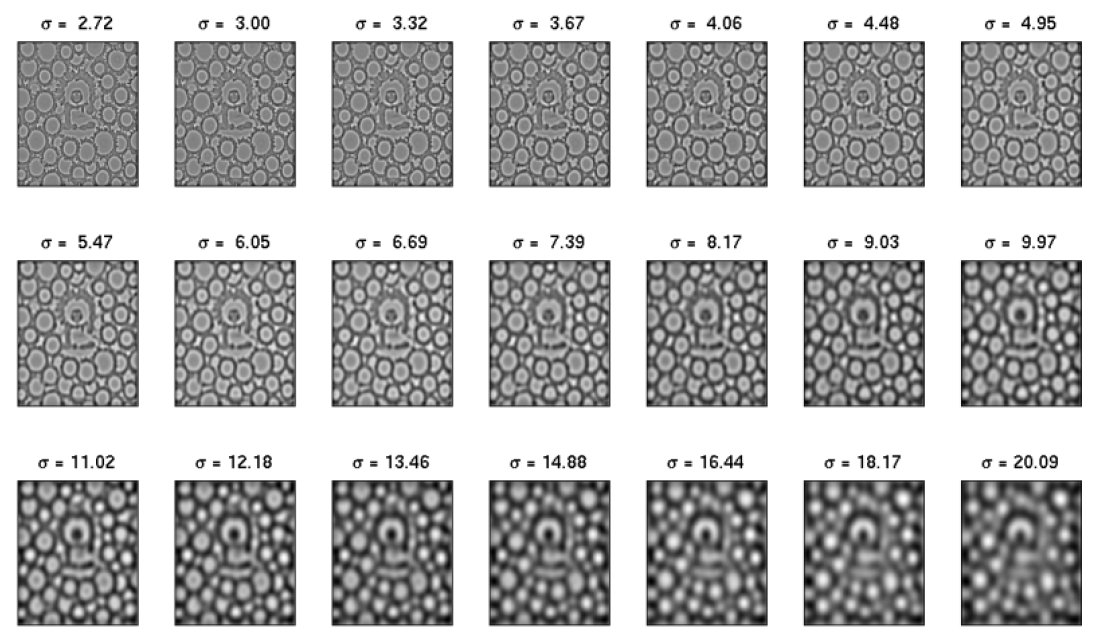
\includegraphics[width=\textwidth]{images/chap5/LOG_norm}

\begin{itemize}
    \item Factor $\sigma^2$ req. for true \textbf{scale invariance}
    \item Structures appear and vanish (bandpass behavior)
    \item At \textbf{characteristic scale} of feature, magnitude of NLoG takes extrema (min. or max.)
    \item Computing extrema in scale and space provides \textbf{location} and \textbf{scale} of features
    \item Simple case: extrema of NLoG can be found by comparing with direct neighbors in scale and space (doesn't have to be this way!)
\end{itemize}

\subsection{Step 2: Accurate Localisation of Key Points}

\textbf{Step 2a: Sub-pixel refinement}

Determine sub-pixel location of extemas by performing second order Taylor Expansion (poly. fit) around each feature point $\mathbf{x_i} = (x_i, y_i, \sigma_i)$ for distance $\mathbf{h}$:

$$D(\mathbf{x_i} + \mathbf{h}) \approx D(\mathbf{x_i}) + \nabla D(\mathbf{x_i})^T \mathbf{h} + \frac{1}{2} \mathbf{h}^T H(x_i) \mathbf{h}$$

$\nabla D$ being the gradient, $H = H(D)$ the hessian of the scale-space function, which can be approx. locally by central differences using neighbor pixels.

\textbf{Hessian:} $3\times 3$ symmetric matrix of mixed second derivative (is a tensor), the \textbf{gradient} a $3\times 1$ column vector.

\textbf{Condition} for extrema locations is given by setting the \textbf{derivative of quadratic approx. to zero}: $ \nabla D(\mathbf{x_i}) + H(\mathbf{x_i}) \mathbf{h} = 0$. Offset to extremum is given b $\hat{\mathbf{h}} = - H(\mathbf{x_i})^{-1} \nabla D(\mathbf{x_i})$. \textbf{New location} is $\hat{\mathbf{x_i}} = \mathbf{x_i + \hat{h}}$. Replacing $\mathbf{h, \hat{h}}$ in the function yields

$$D(\mathbf{\hat{x}_i}) = D(\mathbf{x_i}) + \frac{1}{2} \nabla D(\mathbf{x_i})^T \mathbf{\hat{h}}$$

\textbf{Improves accuracy of feature locations w.r.t. scale and location!}

\textbf{Step 2b: Elimate weak detections}

Discard iff $D(\mathbf{\hat{x}_i})$ is below threshold (paper use 0.03). Eliminates unreliable features in regions with low contrast.

\textbf{Step 2c: Elimination of unstable features}

Based on \textbf{principal curvatures:} Measures how surface bends in different directions. \textbf{Goal:} Smallest ad largest bending have same sign and magnitude, then extremum is stable.

Eigenvalues $\lambda_1 \geq \lambda_2$ of spatial Hessian $H_2 = \left[ \begin{matrix}
D_{xx} & D_{xy} \\
D_{yx} & D_{yy}
\end{matrix}\right]$

proportional to principal curvatures at $x,y$. For small ratios $r = \lambda_1 / \lambda_2 \geq 1$, the following expr. is minimized (does not need eigenvalue computation directly): $$\mathcal{K} = \dfrac{trace(H_2)^2}{det(H_2)} = \dfrac{(\lambda_1 + \lambda_2)^2}{\lambda_1\lambda_2} = \dfrac{(r+1)^2}{r} = r + 2 + \frac{1}{r}$$.

Discarding features iff, $det(H_2) < 0$, "saddle points" instead of extrema, $det(H_2) = 0$ no extrema. $\mathcal{K} > 10$, looks like ridge/valley instead of peak!

\subsection{Step 3: Assignment of dominant orientations}

\textbf{HoG:} For each feature point $\mathbf{x_i}$. Computed from gradients for $\hat{\sigma}_i$. Histogram using 36 bins (360°), weighted by magnitude of gradient and with gaussian centered at $(\hat{x}_i, \hat{y}_i)$, with STD $1.5\hat{\sigma}_i$.

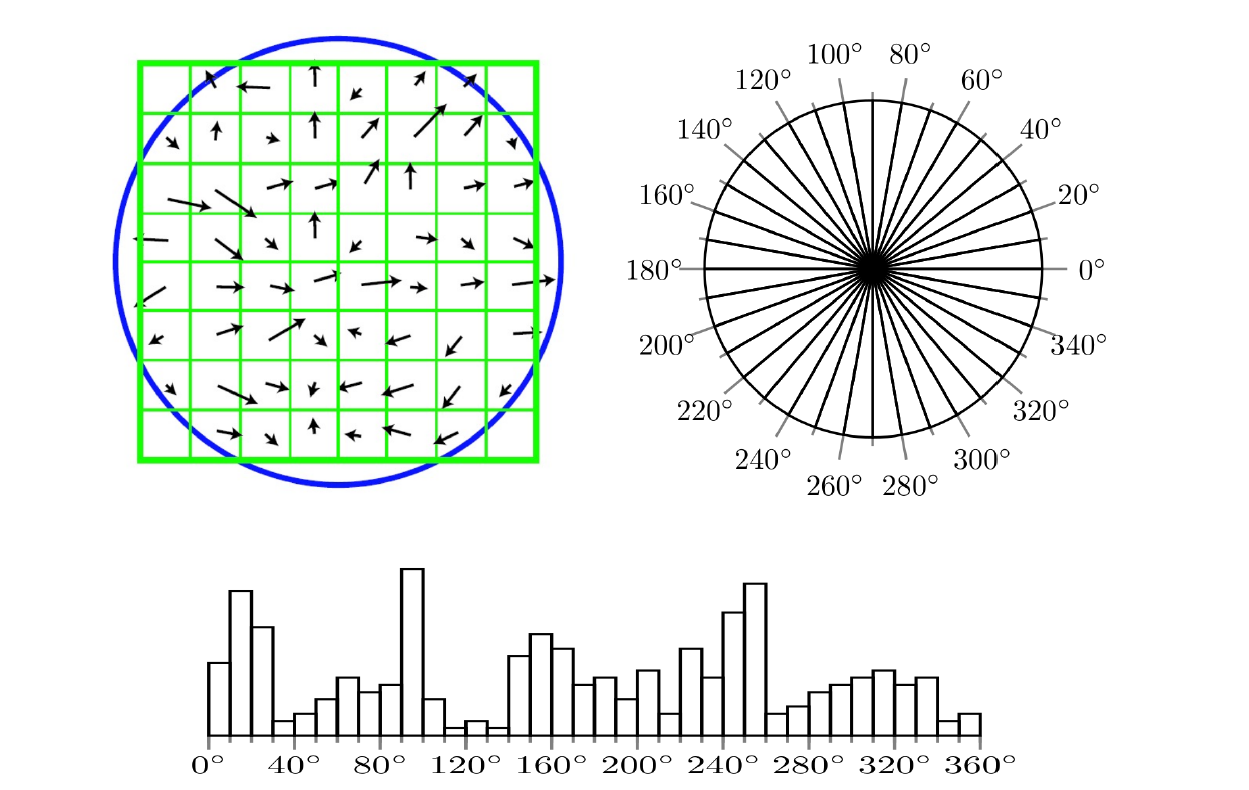
\includegraphics[width=\textwidth]{images/chap5/HoG}

Arrows: Gradients in circular neighborhood. \textbf{Blue} circle, $3\sigma$ of gaussian use for weighting. Histogram is created by angles. \textbf{Dominant} orientation is given by largest entry!

\textbf{Feature cloning for multiple dominant orientations:} Separate feature point for every entry that is above $80\%$ of value of dominant orientation. Sub-bin refinement is applied as well (1D).

Assignment looks like

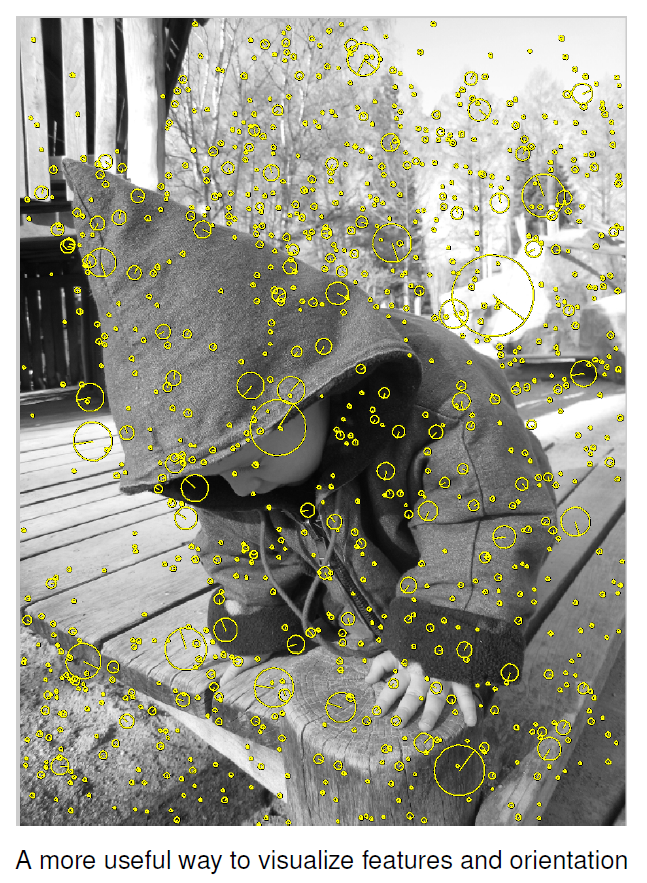
\includegraphics[width=.4\textwidth]{images/chap5/ori_asg}

\textbf{Step 4: Computation of suitable key point descriptors}

\textbf{Goal:} Unique representation of feature points by characteristic vectors.

\textbf{Block of HoGs:} Same as in orientation assignment (consider scale and location, mag. weighting, gaussian weighting). \textbf{Additionally}, sample location and gradient directions and rotate patch into "default" direction. Neighborhood divided in 16 blocks of $4\times 4$. Histograms using 8 bins, covering $45°$.

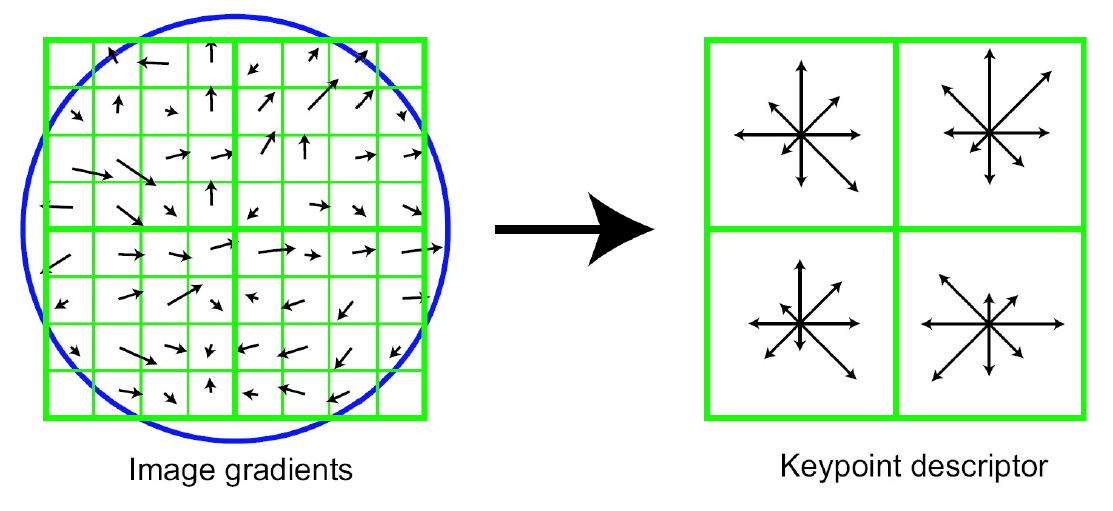
\includegraphics[width=.6\textwidth]{images/chap5/block_hog}

Example 4 blocks of $4\times 4$, i.e., 64 features. SIFT uses 16 blocks!. Right pictures is the keypoint descriptor as \textbf{HoG}.

\textbf{Problems:} Slight rotations/translations contribute same gradients to different bins (possibly).

\textbf{Solution:} Dist. votes of each gradient to neighboring bins and four neighboring blocks based on angular and spatial distance.

\section{SIFT Descriptor}

Stored for every feature, size 128 with 8 entries for 16 block histograms, for matching FD are compared computing euclidean norm of differences.

\textbf{Successful SIFT:}

\begin{itemize}
    \item Invariance under scaling, shift and rotation (information computed at characteristic scale by dominant orientation)
    \item Invariance under affine illumination changes (gradient is invariant for additive illumination, normailzation makes it invariant for multiplicative illumination changes)
    \item up to 60 degrees out of plane rotation demonstrated to still work quite well!
\end{itemize}


















\chapter{Coordinate Transformations and Alignment}
Want to align images, find their geometric relationship. If they don't align we need to perform transformations s.t. they align properly.

\section{Coordinate Transformations}

Transform image according to map $T : \mathbb{R}^2 \rightarrow \mathbb{R}^2$.

\textbf{How to generate transformed image?}

Given image $f$ in region $\Omega \subset \mathbb{R}^2$, mapping $T: \Omega \rightarrow \mathbb{R}^2$, we want to generate image $g$ in region $\Omega' \subset \mathbb{R}^2$, s.t., $g(T(\mathbf{p})) = f(\mathbf{p}), $ for all $\mathbf{p} \in \Omega$. $T$ might map outside the region...

\textbf{Naive approach (Forward Splatting):} Compute location for every pixel, throw away the pixel if it isn't in the new region and copy it to $g$ if it is.

\textbf{Problems with forward splatting:} What if $\mathbf{p'}$ not on integer pixel location?

\begin{itemize}
    \item Round coordinates, putting it to the nearest pixel - result: sever aliasing, unstable
    \item Better: Distribute among neighbors with weighting kernel
    \item Keep track of per-pixel weights, normalize
    \item Called \textbf{splatting}, suffer from aliasing and blur!
\end{itemize}

Appearance of cracks and holes, especially when magnifying..

\textbf{Implementation II: Inverse Warp}

Approach: Compute location $\mathbf{p} = T^{-1}(\mathbf{p'})$, boundary conditions apply, copy value again. Needs knowledge about the inverse map.

\textbf{Concentrate on linear maps, can be represented only with a few parameters!}

\subsection{Linear Transformations}

Map which can be written as $T(\mathbf{p}) = A\mathbf{p}$, $A \in \mathbb{R}^{2\times 2}$.

Common linear map: \textbf{Scaling} - $A = \left[\begin{matrix}s_x & 0 \\ 0  & s_y \end{matrix}\right]$, $s_x , s_y \neq 0$. \textbf{Rotation} - $A = \left[\begin{matrix}\cos \Theta & -\sin \Theta \\ \sin \Theta  & \cos \Theta \end{matrix}\right]$

Compositions of $n$ linear maps $T_1, \dots, T_n$ can be written as concatenation of application in the right order $T_n(\dots(T_1(\mathbf{p})\dots ) = A_n A_{n-1} \dots A_1 \mathbf{p} = A \mathbf{p}$. Composition of linear maps is linear, duh.

\textbf{SVD:} Can get all information about linear maps by looking at \textbf{SVD}. $A = U \Sigma V^T$, we know $A$ maps $V$ onto scaled $U$. Another interpretation: Linear trans. can be written as \textbf{rotation} $V^T$ followed by scaling $\Sigma$, followed by another \textbf{rotation} $U$.

\textbf{Properties:} \textit{Origin maps to origin, Lines map to lines, parallel lines remain parallel, ratios are preserved, closed under composition}!

\subsection{Affine Transformations}
Translation missing in linear trans. Hence, we generalize to \textbf{affine} transformation, applying linear trans. $A$ and afterwards translation $\mathbf{t}$, i.e., $T(x) = Ax + \mathbf{t}$.

\textbf{Properties:} \textit{Origin is not mapping to origin}, \textbf{otherwise same as linear}.

\textbf{Special cases of  Affine Transformations:} (Important, hence memorize these)

\begin{itemize}
    \item \textbf{Translation} - $A = I_2$, two degs. of freedom. I.e. only $\mathbf{t}$ changes the image.
    \item \textbf{Euclidean (rigid motion)} - $A$ pure rotation, three degrees of freedom (from translation we have two and one from rotation, i.e., the angle $\phi$)
    \item \textbf{Similarity} - $A = sR$, $R$ rotation and $s > 0$ scaling. Three DoFs from before + 1 from scaling, i.e., \textbf{4 DoF!}
    \item \textbf{Area Preserving} - $det(A)  = 1$, areas stay the same, \textbf{5 DoF!}
\end{itemize}

\subsection{Corresponding matrix groups}

Group of all invertible matrices is \textbf{general linear group}: $GL(2) = \{A \in \mathbb{R}^{2\times 2} : det(A) \neq 0\}$, operation is matrix multiplication (concatenating maps).

Subgroup of \textbf{area preserving maps}:  $SL(2) = \{A \in \mathbb{R}^{2\times 2} : det(A) = 1\}$

\textbf{Pure rotation} is  $SO(2) = \{A \in \mathbb{R}^{2\times 2} : det(A) = 1 \wedge A^T A = AA^T = 1\}$, which is a subgroup of the \textbf{orthogonal group} (allows reflection): $O(2) = \{A \in \mathbb{R}^{2\times 2} : A^T A = AA^T = 1\}$

\subsection{Moving to homogenous coordinates}

Make coordinates \textbf{homogenous} by adding a coordinate. Points on line $[wx \ wy \ w]^T$ are identified, equality holds by scaling factor $w$.

Affine maps: $T(\mathbf{p}) = A \mathbf{p} + \mathbf{t}$, Homogenous: $\widehat{T(\mathbf{p})} = \left[\begin{matrix}
    A & \mathbf{t} \\
    0 & 1
\end{matrix}\right]\left[\begin{matrix}
    \mathbf{p}\\
    1
\end{matrix}\right]$

\textbf{Two new parameters}: $H = \left[\begin{matrix}
    A & \mathbf{t} \\
    b^T & 1
\end{matrix}\right]$, i.e., $b$ which is a two row vector. The map is called homography (projective transformation or planar perspective map).

\subsection{Understanding geometry of homographies}

\textbf{Special case:} $H = \left[\begin{matrix}
1 & 0 & 0 \\ 0 & 1 & 0 \\ -\frac{1}{f} & 0 & 1 
\end{matrix}\right]$, with $f \neq 0$. Then applied to a point, the image of $[x \ y]^T$ is $\left[ \begin{matrix}x \\ y \\ -\frac{x}{f+1}\end{matrix} \right] \approx
\left[ \begin{matrix}\frac{fx}{f-x} \\ \frac{fy}{f-x}\end{matrix} \right]$, if $x = f$, denominator $= 0$ hence point at infinity.

\textbf{How about lines parallel to the y-axis?:} $H$ the same, let $t \in \mathbb{R}$ and $x_0$ constant, then for $[x_0 \ t \ 1]^T$, mapping is $\left[ \begin{matrix}\frac{fx_0}{f-x_0} \\ \frac{ft}{f-x_0}\end{matrix} \right]$, so we get again vertical lines. But the x-coord. changes non linearly, i.e. the distances between two vertical lines may differ!

\textbf{Horizontal lines:} $H$ again, $[t \ y_0 \ 1 ]^T, t \in \mathbb{R}$, we get $\left[ \begin{matrix}\frac{ft}{f-t} \\ \frac{fy_0}{f-t}\end{matrix} \right]$, with $t \rightarrow \infty$, we get $[-f \ 0]^T$, a point at infinity in x-direction (vanishing point).

\textbf{Special case: Two vanishing points}

$H = \left[\begin{matrix}
1 & 0 & 0 \\ 0 & 1 & 0 \\ -\frac{1}{f_x} & -\frac{1}{f_y} & 1 
\end{matrix}\right], f \neq 0, f_x = f_y = 2000$, vertical lines are now not vertical but intersect a vanishing point as  well, since we get for a point $\left[\begin{matrix}
-\frac{f_x f_y x}{f_y x + f_x y - f_x f_y} \\ -\frac{f_x f_y y}{f_y x + f_x y - f_x f_y}
\end{matrix}\right]$.

\textbf{Special case: Moving image before hand}

$H = \left[\begin{matrix}
1 & 0 & t_1 \\ 0 & 1 & t_2 \\ -\frac{1}{f_x} & 0 & 1 
\end{matrix}\right], f \neq 0$ for a point we get $\left[\begin{matrix}
-\frac{fx + ft_1}{f - x} \\ -\frac{fy + ft_2}{f-x}
\end{matrix}\right]$

\subsection{Overview and summary of coordinate transforms}

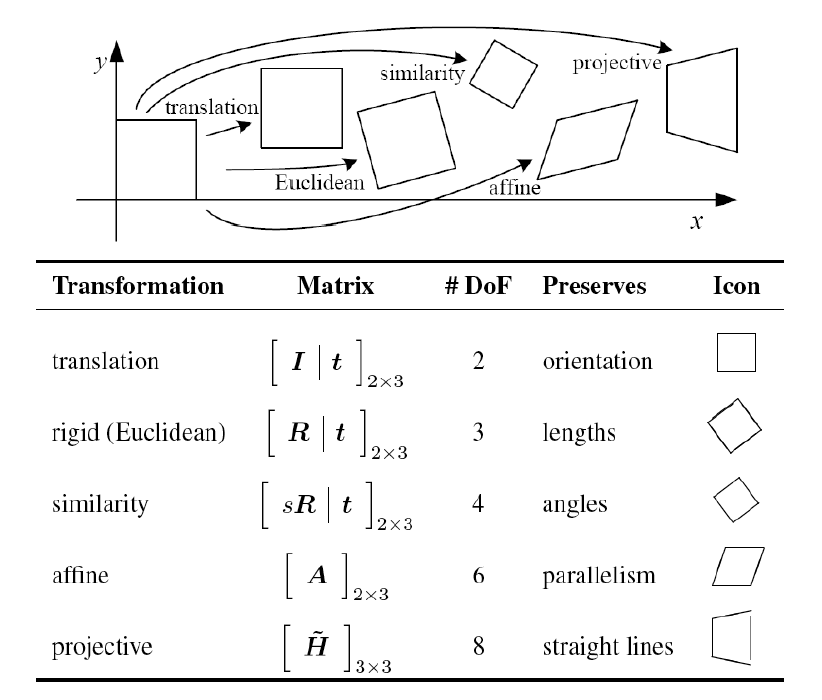
\includegraphics[width=\textwidth]{images/chap5/summ_coord_trans}

\section{Model Fitting I: Least Squares}

From now on, we want to estimate homographies using \textbf{correspondance information}

\textbf{Homography} between two image planes $\Omega, \Omega', \mathbf{p}_i \in Omega, \mathbf{p}'_i \in \Omega', 1 \leq i \leq m$, estimating $H =  \left[\begin{matrix}
h_{11} & h_{12} & h_{13} \\
h_{21} & h_{22} & h_{23} \\
h_{31} & h_{32} & 1 \\
\end{matrix}\right]$, giving us \textbf{8 Degrees of Freedom}.

\textbf{Problem:} $H$ defined in proj. coords, which is only correct up to scaling factor!

\textbf{Two equations from one coorespondance:} $\mathbf{p}_i = [x_i \ y_i \ 1]^T$ normalized, $\mathbf{p}'_i = [x'_i \ y'_i \ w'_i]$ not normalized! Then we get a linear system \begin{align*}
    x'_i & = h_{11} x_i + h_{12} y_i + h_{13} \\
    y'_i & = h_{21} x_i + h_{22} y_i + h_{23} \\
    w'_i & = h_{31} x_i + h_{32} y_i + 1
\end{align*}, from which we get the following two equations: \begin{align*}
    \frac{x'_i}{w'_i} (h_{31} x_i + h_{32} y_i + 1) - h_{11} x_i - h_{12} y_i - h_{13} & = 0 \\
    \frac{y'_i}{w'_i} (h_{31} x_i + h_{32} y_i + 1) - h_{21} x_i - h_{22} y_i - h_{23}
\end{align*}, i.e., we divide by $w'_i$ and intersect with $0$.

\begin{itemize}
    \item Correspondance leads to two equations
    \item \textbf{Problem:} Overfitting/Overdetermining by having more equations than variables
    \item 2 times correspondences equations for $8$ unknowns..
    \item Frequent problem in science!
\end{itemize}

The corresponding linear system (by correspondences) is:

$\left[\begin{matrix}
& & & & \vdots & & & \\
-x_i & -y_i & -1 & 0 & 0 & 0 & \frac{x'_i}{w'_i}x_i & \frac{x'_i}{w'_i} y_i \\
0 & 0 & 0 & -x_i & -y_i & -1 & \frac{y'_i}{w'_i}x_i & \frac{y'_i}{w'_i} y_i \\
& & & & \vdots & & &
\end{matrix}\right]\left[
\begin{matrix}
h_{11} \\h_{12} \\h_{13} \\h_{21} \\h_{22} \\h_{23} \\h_{31} \\h_{32}
\end{matrix}\right] = \left[
\begin{matrix}
\vdots \\ -\frac{x'_i}{w'_i} \\ -\frac{y'_i}{w'_i} \\ \vdots
\end{matrix}\right]
$

\textbf{Considerations}: We have $Ax = b$, looking for $x \in \mathbb{R}^n$ and $ m > n$, we often do not have an exact solution! But we can try to find \textbf{the best fit}.

\textbf{Least Squares:} Minimize distance to $b$ finding $\hat{y} = A\hat{x}$ with $\hat{x} = \mathrm{argmin}_{x\in \mathbb{R}^n} \frac{1}{2} ||Ax - b||^2$. The line from $\hat{y}$ to $b$ is orthogonal to our model, hence lowest distance. In formulas we can get the \textbf{normal equations}: $$A^T (A\hat{x} -b ) = 0 \leftrightarrow A^T A\hat{x} = A^T b$$.

\textbf{Analytic point of view:} Minimizer for $E(x) = \frac{1}{2}||Ax - b||^2$, can use the gradient which is $\nabla E(x) = A^T (Ax - b)$, i.e. the same as the geometric solution.

\textbf{Solution to the normal equations:} (\textbf{if $A^T A$ has an inverse..}) Use $SVD$, i.e. $A = U\Sigma V^T$ which reduces \textbf{normal equations} to $$\Sigma^2 V^T \hat{x} = \Sigma U^T b$$. 

With left-inverse of $\Sigma$, $\Sigma^2$ vanishes, it can be found inverting every singular value, i.e. $\Sigma^+ = \mathrm{diag}(\sigma_1^{-1}, \dots, \sigma_k^{-1}, 0 , \dots , 0)$, so we get $\Sigma^+ \Sigma = I$, with $\hat{x} = V \Sigma^+ U^T b$ and $A^+ = V \Sigma^+ U^T$ being the \textbf{pseudo inverse} of $A$!

\textbf{Weighted least squares:} Add weights $\sqrt{w_i}$ to the correspondences. Solution is same as before..

\textbf{Problems:} \begin{itemize}
    \item outliers make for bad results
    \item one strong outlier may destroy the whole result
\end{itemize}

\section{Model Fitting II: RANSAC}

\textbf{RANdom SAmple Consensus:} \begin{itemize}
    \item {Repeat $N$ times
    \begin{itemize}
        \item Select random subset of samples
        \item Compute model
        \item Compute error between samples and model
        \item Count \textbf{inliers} by using \textbf{fixed threshold}
    \end{itemize}        
    }
    \item Refit model using largest inlier set found during the $N$ iterations
\end{itemize}

\textbf{Parameters:} 

\textbf{1: Number of points selected for model fitting:} Choose minimum, since
\begin{itemize}
    \item Faster fits, more iterations in same amount of time
    \item More likely to randomly select only inliers
    \item \textbf{Tradeoff:} Initialization may not be good for minimal sample size
\end{itemize}

\textbf{2: Threshold:} Choose with 95\% probability for an inlier to stay below threshold. \textbf{Example:} Gaussian noise with $\sigma$ expected on data, 95\% of inliers will be within $2\sigma$, 99\% within $3\sigma$.

\textbf{3: Number $N$ of hypothesis trials:} 

Choose $N$ with $p$ so that one random sample is free from outliers. Given \textbf{percentage of outliers in the data $e$} we have \begin{align*}
    (1- (1-e)^s)^N & = 1 - p \\ N & = \frac{\log(1-p)}{\log(1-(1-e)^s)}
\end{align*}

The higher $s$ is chosen, the faster the number $N$ grows in relation to the outlier amount in percent. \textbf{Works well for ratios less than 50\%}!

\textbf{Problem:} $e$ unknown, hence we need adaptive approach: Start with $count = 0, e= 1$ and as long as $N > count$ \begin{itemize}
    \item Perform RANSAC as usual
    \item $e \leftarrow \mathrm{min} (e , 1 - \frac{numInliers}{numPoints})$
    \item $N \leftarrow \frac{\log(1-p)}{\log(1-(1-e)^s)}$
    \item $count \leftarrow count + 1$
\end{itemize} , i.e., we update $e$ if we find a better value of $e$ out of the inliers and point amount we look at, then $N$ can be updated.

\textbf{RANSAC on Homography estimation:}

Correspondences agree what $H$ looks like, small outlier amount does not agree.

Approach: \begin{itemize}
    \item Define max number of iterations, otherwise same as adaptive approach
    \item \textbf{In each iteration}: Select 4 correspondences randomly
    \item Compute $H$
    \item Compute error $\epsilon$ for $H$ and correspondences
    \item If the new inliers are more than previously replace everything (also $e$ and $N$ according to adaptive approach)
\end{itemize}

\textbf{PROs and CONs:}
\begin{itemize}
    \item[+] Simple/general
    \item[+] Many applications 
    \item[+] Works well in practice
    \item[-] Several parameters
    \item[-] Not deterministic
    \item[-] Iterative with unknown number $N$
    \item[-] Bad for low inlier ratios
    \item[-] Not always good initialization based on minimum number of samples
\end{itemize}

\textbf{RANSAC} is classic example for \textbf{Voting Scheme}, like \textbf{Hough transform}

\section{Model Fitting III: Hough Transform}

Just a rough look at hough transform..

\begin{itemize}
    \item \textbf{Voting Scheme} for fitting low-parameter models
    \item Detect \textbf{simple} geometric objects, represented by \textbf{very few} parameters (lines,circles)
    \item Assumptions: {\begin{itemize}
        \item Boundaries with large $|\nabla|$
        \item Points satisfy $g(\mathbf{p}, \alpha_1, \dots, \alpha_m) = 0$, $\alpha$ parameters to be determined
    \end{itemize}}
    \item \textbf{Examples:} {\begin{itemize}
        \item Line with normal $\mathbf{n} = (\cos \phi, \sin \phi)$, distance $d$ to origin can be represented as $x\cos \phi + y\sin \phi - d = 0$
        \item Circle with center $(a,b)$ radius $r$ as $|x-a| + |y-b| - r$ = 0
    \end{itemize}}
    \item \textbf{Object rep:} {\begin{itemize}
        \item Work on space of parameters
        \item Points in param space describe different objects in image space
    \end{itemize}}
    \item \textbf{Voting Strategy:} {\begin{itemize}
        \item Detect all edges
        \item Every edge point votes for all params to satisfy the upper equation
        \item Majority rule: parameters of most relevant object gets the mos votes
    \end{itemize}}
    \item \textbf{Advantages:} {\begin{itemize}
        \item No fully connected contours needed
        \item Detects all objects which fit the model
        \item Very robust
    \end{itemize}}
    \item \textbf{Disadvantages:} {\begin{itemize}
        \item Memory requirements and computational effort increases rapidly with parameters
        \item Bad parallelization..
    \end{itemize}}
\end{itemize}

\section{Summary}
\chapter{Lights, Optics, Color}

No need to learn this chapter 8).
\chapter{Cameras}

\section{Real-world cameras}

\textbf{Idea 1:} Piece of film in front of a scene

\textbf{Idea 2:} Add barrier to block off most of the rays (less blurring)

\textbf{The pinhole camera:} 

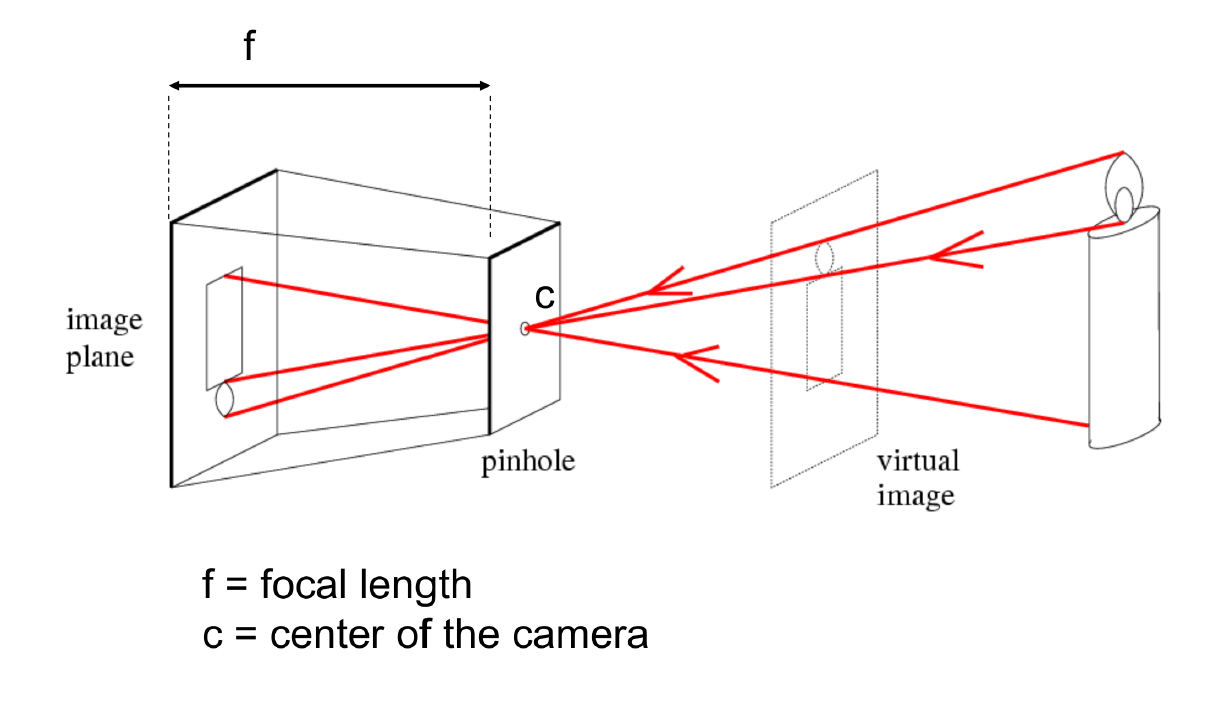
\includegraphics[width=\textwidth]{images/chap7/pinhole}

\textbf{Why lenses?} Pinhole non-zero size, hence object points blurr. Smaller pinhole means \textbf{less blurry}! Can't make arbitrarily small due to physical limitations, i.e., less light goes through, need long exposure, also we have a \textbf{diffraction limit} which means it will ge blurrier at some point.

\textbf{Simple camera design with a single thin lens:}

\textbf{Lens focuses light onto film}: \begin{itemize}
    \item Specific distance at which objects are \textbf{in focus}
    \item Determined by \textbf{focal length}
    \item Points out of focus project to \textbf{circle of confusion}
    \item Larger \textbf{circles of confusion} cause blurr
    \item \textbf{Depth of field} - range in which image appears sharp
\end{itemize}

\textbf{Depth of field and aperture}: Smaller aperture increases range in which object is in focus. Reduces amount of light - need to extend exposure.

\section{Camera models}

Major goal is to extract information of 3D world out of 2D images. Simple case, we consider singe pinhole cameras, i.e., \textbf{monocular vision} which requires \textbf{single view projective geometry}.

\subsection{Pinhole Camera Model}

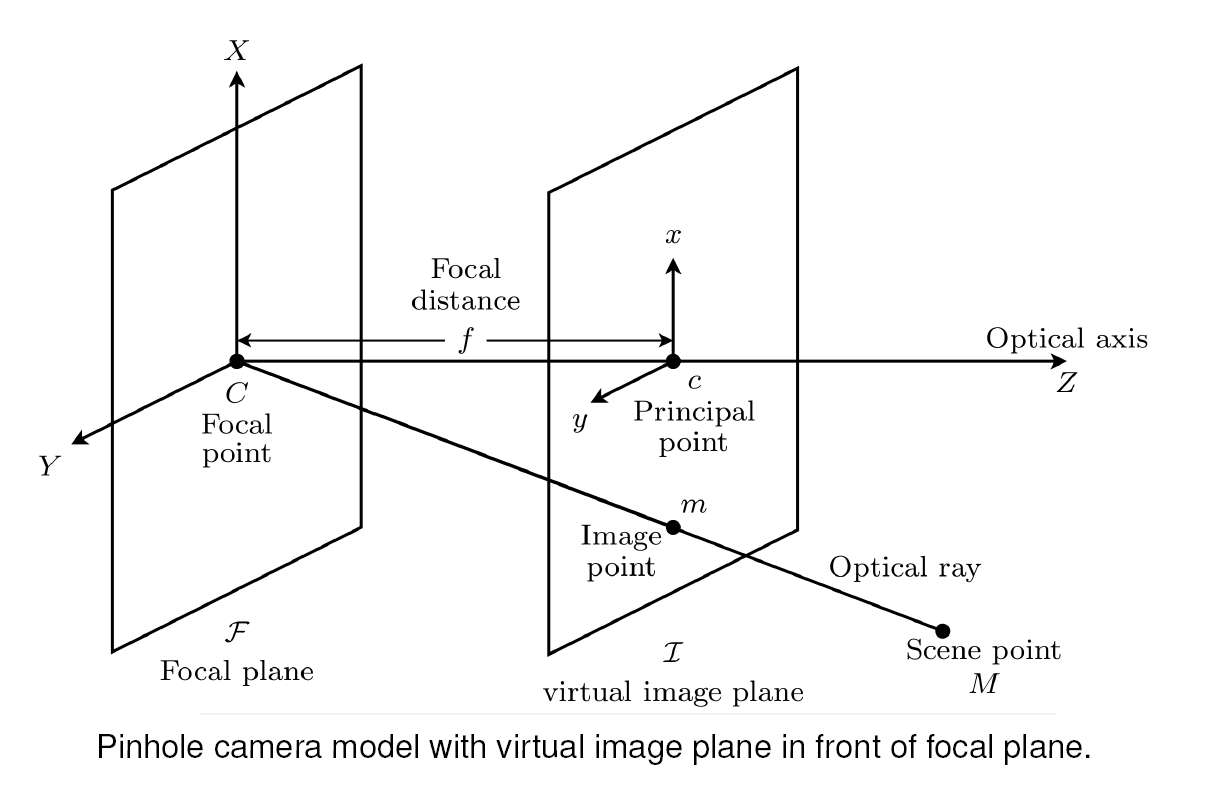
\includegraphics[width=\textwidth]{images/chap7/pinhole_model}

\textbf{Simplified but sufficiently realistic} model of a camera system. Coordinates $(X,Y,Z)$ with origin $C$ map to $m=(x,y)$ with origin $c$.

Notations: \begin{itemize}
    \item $M$, \textbf{scene point}
    \item $C$, \textbf{focal point, optical center}, pinhole location
    \item $m$, \textbf{image point}
    \item $I$, \textbf{image plane}
    \item $F$, \textbf{focal plane}
    \item \textbf{optical axis:} orthogonal to image plane, passes through $C$
    \item \textbf{opical ray:} passes through $M$ and $C$
    \item $f$, \textbf{focal distance}
    \item $c$, \textbf{principal point: intersection} between image plane and optical axis
\end{itemize}

\textbf{Basic geometric relations:} $\frac{x}{X} = \frac{y}{Y} = \frac{f}{Z}$, we see nonuniqueness of projection, since all points on one optical ray with different distances $Z$ are projected to $m = (x,y)$ and we lose depth information.

The previous equation is a nonlinear transformation from 3D to 2D, \textbf{solution?}: \textbf{Lift $m$ to projective space, by adding a coordinate $1$}!

\textbf{Thus}, pinhole projection in homogenous coordinates is projective linear map 
$\mathbb{P}^3 \rightarrow \mathbb{P}^2$: $$\hat{m} = \left[\begin{matrix}
x \\ y \\ 1
\end{matrix}\right] =\left[\begin{matrix}
Zx \\ Zy \\ Z1
\end{matrix}\right] = \left[\begin{matrix}
fX \\ fY \\ Z
\end{matrix}\right] = \underset{P}{\underbrace{\left[\begin{matrix}
f & 0 & 0 & 0 \\ 0 & f & 0 & 0 \\ 0 & 0 & 1 & 0
\end{matrix}\right]}}
\left[\begin{matrix}
X \\ Y \\ Z \\ 1
\end{matrix}\right]$$, with $P$ being the \textbf{Projection Matrix}.

\subsection{Extrinsic Camera Parameters}

Denote position of world coordinates relative to camera coordinates. 3D transformation can be expressed by $4\times 4$ \textbf{matrices}.

\textbf{Translation:} $T = \left[\begin{matrix}
1 & 0 & 0 & t_1 \\ & 0 & 1 & 0 & t_2 \\ 0 & 0 & 1 & t_3 \\ 0 & 0 & 0 & 1
\end{matrix}\right] = \left[ \begin{matrix} I & t \\ 0 & 1 \end{matrix} \right]$,

\textbf{Rotation:} $R = \left[\begin{matrix}
r_{11} & r_{12} & r_{13} & 0 \\ r_{21} & r_{22} & r_{23} & 0 \\ r_{31} & r_{32} & r_{33} & 0 \\ 0 & 0 & 0 & 1
\end{matrix}\right] = \left[\begin{matrix} R & 0 \\ 0 & 1 \end{matrix} \right]$, with $RR^T = R^T R = I_4$, with rotations for

$R_x(\Phi) = \left[\begin{matrix}
1 & 0 & 0 & 0 \\ 0 & \cos \Phi & -\sin \Phi & 0 \\ 0 & \sin \Phi & \cos \Phi & 0 \\ 0 & 0 & 0 & 1
\end{matrix}\right]$, $R_y(\Phi) = \left[\begin{matrix}
\cos \Phi & 0 & -\sin \Phi & 0 \\ 0 & 1 & 0 & 0 \\ \sin \Phi & 0 & \cos \Phi & 0 \\ 0 & 0 & 0 & 1
\end{matrix}\right]$, $R_z(\Phi) = \left[\begin{matrix}
\cos \Phi & -\sin \Phi & 0 & 0 \\ \sin \Phi & \cos \Phi & 0 & 0 \\ 0 & 0 & 1 & 0 \\ 0 & 0 & 0 & 1
\end{matrix}\right]$

\textbf{Rotation and translation} does \textbf{not commute}!

We have \textbf{3 DoF} for translation and \textbf{3 DoF} for rotation (1 angle per axis).

\subsection{Intrinsic Camera Parameters}

Describes transition from image coordinates in world units to pixel coordinates and therefore \textbf{the geometry of the image plane inside the camera}.

\textbf{Frequent properties}: \begin{itemize}
    \item Origin of the image plane can be located in another point than the \textbf{principal point}
    \item Let principal point of new coordinate system be in $(u_0, v_0)$
    \item $(u,v)$ measured in pixel units has e.g., $k,l$ pixels per meter.
\end{itemize}

From these four intrinsic parameters we get the matrix transformation $$\left[\begin{matrix}u \\ v \\ 1 \end{matrix} \right] = \left[\begin{matrix}k & 0 & u_0 \\ 0 & l & v_0 \\ 0 & 0 & 1 \end{matrix} \right]\left[\begin{matrix}x \\ y \\ 1 \end{matrix} \right]$$, which describes transition from projective coordinates to pixel coordinates. $k,l$ scaling and $u_0 , v_0$ for translation.

If the coordinate system is \textbf{skewed}, i.e., v-axis has an angle $\Theta \neq 90°$ to the u-axis we get:
$$\left[\begin{matrix}u \\ v \\ 1 \end{matrix} \right] = \left[\begin{matrix}k & -k \cot\theta & u_0 \\ 0 & l/\sin\theta & v_0 \\ 0 & 0 & 1 \end{matrix} \right]\left[\begin{matrix}x \\ y \\ 1 \end{matrix} \right]$$

In practice skew is assumed to be $0$! Also pixel sizes $k,l$ from manufacturers can generally be trusted.

\textbf{Intrinsic matrix, note on units:} $H$ and $P$ often multiplied to form single \textbf{intrinsic matrix} $K$, \textbf{which transforms from camera coordinates to homogenous pixel coordinates}:
$$K = \underset{H}{\underbrace{\left[\begin{matrix}k & -k \cot\theta & u_0 \\ 0 & l/\sin\theta & v_0 \\ 0 & 0 & 1 \end{matrix} \right]\left[\begin{matrix}x \\ y \\ 1 \end{matrix} \right]}} \underset{P}{\underbrace{\left[\begin{matrix} f & 0 & 0 & 0 \\ 0 & f & 0 & 0 \\ 0 & 0 & 1 & 0\end{matrix}\right]}} = \left[\begin{matrix}kf & -kf \cot\theta & u_0  & 0\\ 0 & lf/\sin\theta & v_0 & 0 \\ 0 & 0 & 1 & 0 \end{matrix} \right]$$

\textbf{Focal length $f$} usually given in physical unit (meters) and as $k,l$ (pixels per meter).

\textbf{Note:} Only depends on \textbf{products} $\alpha = kf , \beta = lf$, \textbf{magnification} of the system measured in pixels.

\subsection{Complete Pinhole Camera Model}

Combination of extrinsic and intrinsic parameters to map from \textbf{homogenous world coordinates} to \textbf{homogenous pixel coordinates} is given by:

$$\left[\begin{matrix}
Zu \\ Zv \\ Z
\end{matrix}\right] = \underset{=:\Pi}{\underbrace{KTR}} \left[\begin{matrix}
X_W \\ Y_W \\ Z_W \\ 1
\end{matrix}\right]$$

$K, 3\times 4$ intrinsic matrix, $R, 4\times 4$ rotation matrix, $T, 4\times 4$ translation matrix. Te \textbf{perspective projection matrix} complete describes the camera model with \textbf{11 DoF}, due to arbitrary scale factors from homgenous coordinates: $\Pi = \left[\begin{matrix}
    \pi_{11} & \pi_{12} & \pi_{13} & \pi_{14} \\
    \pi_{21} & \pi_{22} & \pi_{23} & \pi_{24} \\
    \pi_{31} & \pi_{32} & \pi_{33} & \pi_{34}
\end{matrix}\right]$. 

\textbf{Simplification} with the \textbf{affine} camera model is given by $\Pi_{affine} = \left[\begin{matrix}
    \pi_{11} & \pi_{12} & \pi_{13} & \pi_{14} \\
    \pi_{21} & \pi_{22} & \pi_{23} & \pi_{24} \\
    0&0&0&Z_{const}
\end{matrix}\right]$, if the scene points approx. have same distance $Z_{const}$ and has \textbf{6 DoF} since the 8 parameters are not independent. The mapping \textbf{is completely linear}.

\section{Geometry of perspective projection}

\textbf{Properties:}\begin{itemize}
    \item \textbf{Many-to-one}: Points along ray map to same point
    \item \textbf{Points map to points}: Projection on focal plane is undefined
    \item \textbf{Lines map to lines:} Lines through focal point (visual rays) project to a point.
    \item \textbf{Convex sets in 3D map to convex sets in 2D}
\end{itemize}

\subsection{Vanishing points}

Lines parallel in world coordinates vanish in a single point.

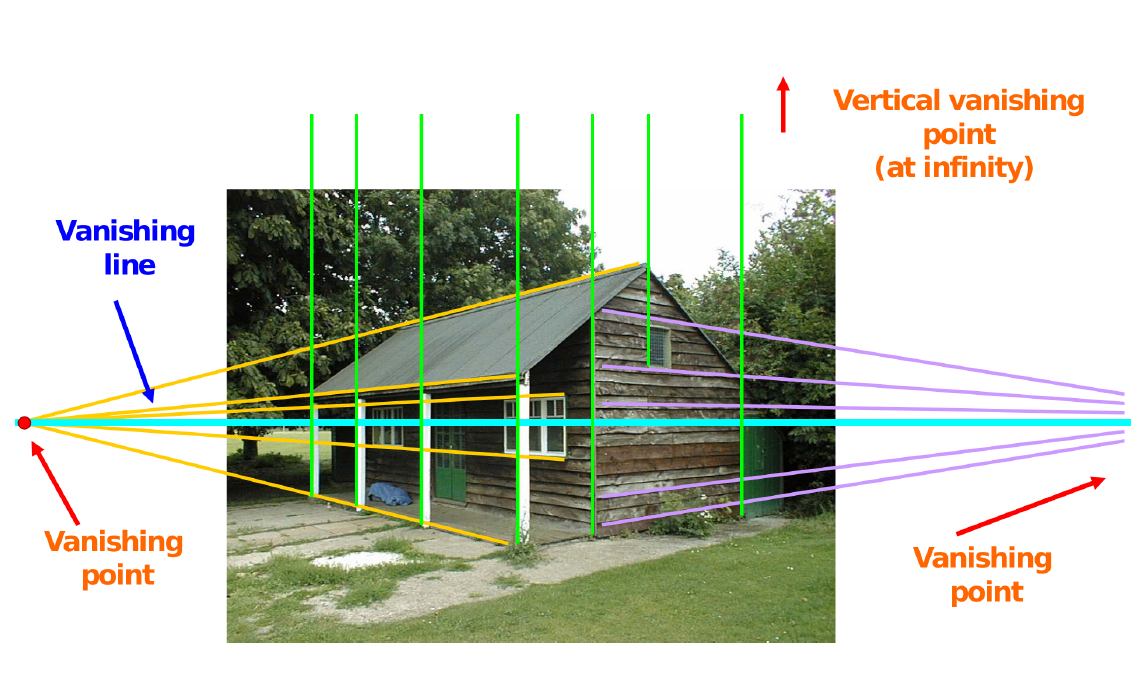
\includegraphics[width=\textwidth]{images/chap7/vanishing_points}

\textbf{Vanishing lines} are what lines parallel to a plane converge to (ground plane -> horizon).

\textbf{Computation 1:} Given line in world coordinates $Mt = \rectmat{x_0 \\ y_0 \\ z_0} + \rectmat{\alpha \\ 0 \\ 1}t$ calculate projection into homogeneous coordinates:

$$PM_t = \rectmat{f&0&0&0 \\ 0&f&0&0 \\ 0&0&1&0} \rectmat{x_0 + \alpha t \\ y_0 \\ z_0 + t \\ 1} = \rectmat{f(x_0 + \alpha t) \\ fy_0 \\ z_0 + 1} \hat{=} \rectmat{\frac{f(x_0 + \alpha t)}{z_0 + t} \\ \frac{fy_0}{z_0 + t} \\ 1}$$. To calculate the vanishing point we have to calculate the limit for $t \rightarrow \infty$:

$$\lim\limits_{t\rightarrow \infty} mt = \lim\limits_{t\rightarrow \infty}\rectmat{\frac{f(x_0 + \alpha t)}{z_0 + t} \\ \frac{fy_0}{z_0 + t} \\ 1} = \lim\limits_{t\rightarrow \infty}\rectmat{\frac{f\alpha t}{z_0 + t} \\ 0 \\ 1} = \lim\limits_{t\rightarrow \infty}\rectmat{\frac{f\alpha t}{t(\frac{z_0}{t} + 1)} \\ 0 \\ 1} = \rectmat{f\alpha \\ 0 \\ 1}$$

\textbf{Computation 2:} Compute the horizon, the set of all vanishing points of lines parallel to the ground plane. A line on the ground plane can be written as a line where the the y-coordinate is not change by parameter $t$:

$Mt = \rectmat{x_0 \\ y_0 \\ z_0} + \rectmat{\alpha \\ 0 \\ \beta}t$, going through the same process as before, i.e. multiplying the matrices we get $$m_t = \rectmat{f&0&0&0 \\ 0&f&0&0 \\ 0&0&1&0} \rectmat{x_0 + \alpha t \\ y_0 \\ z_0 + \beta t \\ 1}  \hat{=} \rectmat{\frac{f(x_0 + \alpha t)}{z_0 + \beta t} \\ \frac{fy_0}{z_0 + \beta t} \\ 1}$$

calculating the limit of $t\rightarrow \infty$, we get for the horizon:

$$\lim\limits_{t\rightarrow \infty} mt = \lim\limits_{t\rightarrow \infty}\rectmat{\frac{f(x_0 + \alpha t)}{z_0 + \beta t} \\ \frac{fy_0}{z_0 + \beta t} \\ 1} = \lim\limits_{t\rightarrow \infty}\rectmat{\frac{f\alpha t}{z_0 + \beta t} \\ 0 \\ 1} = \lim\limits_{t\rightarrow \infty}\rectmat{\frac{f\alpha t}{t(\frac{z_0}{t} + \beta)} \\ 0 \\ 1} = \rectmat{\frac{f\alpha}{\beta} \\ 0 \\ 1}$$

\textbf{Computation 3:} The camera moves up $C$ units in world coordinates. By the last result we have mathematical prove that the horizon stays \textbf{stationary}!

\textbf{Computation 4:}  Optical center fixed, camera rotated 15 degrees around X-axis. Recalculating all possible directions: $$d'(\alpha, \beta) = R_X(\Phi)d(\alpha,\beta) = \rectmat{1 & 0 & 0 & 0 \\ 0 & \cos \Phi & -\sin \Phi & 0 \\ 0 & \sin \Phi & \cos \Phi & 0 \\ 0 & 0 & 0 & 1} \rectmat{\alpha \\ 0 \\ \beta \\ 1} = \rectmat{\alpha \\ -\beta \sin\Phi \\ \beta \cos \Phi \\ 1}$$, this is only the new direction vector, we need to calculate the horizon using this direction vector, as we've done before, going through all calculations we end up at the horizon $$\rectmat{\frac{f\alpha}{\beta\cos\Phi} \\ -\frac{f\sin\Phi}{\cos\Phi} \\ 1} = \rectmat{\frac{f\alpha}{\beta\cos\Phi} \\ -f \tan \Phi \\ 1}$$. In this example the horizon \textbf{moves up} $-\tan(-15°) * f) = 0.2679 * f$ pixels.

\subsection{Perspective distortion}

\textbf{Center of mass in 3D does not map to center of mass in 2D}, i.e., for spheres we get ellipses if they are not the center of the image.

\textbf{Are homographies given when} \begin{itemize}
    \item Translating cameras: Not always, objects can get in front of the scene
    \item Capturing images of a plane: Yes
    \item Rotation: Yes
\end{itemize}

\textbf{Why are planes homographies?} We can assume \textbf{WCS} is chosen, s.t. the plane is parametrized in world coordinates with $[p \ q \ 0 \ 1]^T$. Applying $PRT$ on this point we get a homography.

\textbf{Punchline 1:} Planar surfaces in 3D, reduces projection to a 2D to 2D transformation.

\textbf{Punchline 2:} Transformation is invertible!

\textbf{Why is rotation of the camera still homography?} Let $\rectmat{u \\ v \\ 1} \hat{=} K \rectmat{X \\ Y \\ Z}$ be the primary projection. When rotated we can write $\rectmat{u' \\ v '\\ 1} \hat{=} KR \rectmat{X \\ Y \\ Z} = KRK^{-1}K \rectmat{X \\ Y \\ Z} \hat{=}  KRK^{-1} \rectmat{u \\ v \\ 1}$

$KRK^{-1}$ is the homography between images (called "conjugate relation").

\section{Pinhole camera calibration}

\textbf{What needs to be done?} \begin{itemize}
    \item Determine the \textbf{5 intrinsic} and \textbf{6 extrinsic} parameters
    \item Many algos proposed
    \item \textbf{Basic idea:} Investigate image of \textbf{known} size and shape
    \item Identified point corresponds to 2 constraints
    \item For 11 parameters we need 6 correspondences
    \item Considering more points, makes estimation less sensitive w.r.t. errors
\end{itemize}

\subsection{Basic equations}

\textbf{Input:} We have $k$ correspondences (for which we know the world to image correspondences)

\textbf{Output:} Perspective projection matrix $\Pi = \left[\begin{matrix}
    \pi_{11} & \pi_{12} & \pi_{13} & \pi_{14} \\
    \pi_{21} & \pi_{22} & \pi_{23} & \pi_{24} \\
    \pi_{31} & \pi_{32} & \pi_{33} & \pi_{34}
\end{matrix}\right]$, with $$\widehat{\rectmat{u^i \\ v^i}} = \rectmat{u^i \\ v^i \\ 1} \hat{=} \rectmat{Z^i u^i \\ Z^i v^i \\ Z^i} = \rectmat{\pi_{11} & \pi_{12} & \pi_{13} & \pi_{14} \\
    \pi_{21} & \pi_{22} & \pi_{23} & \pi_{24} \\
    \pi_{31} & \pi_{32} & \pi_{33} & \pi_{34}} \rectmat{X^i_w \\ Y^i_w \\ Z^i_w \\ 1}$$

\textbf{Problem}: We do not know $Z$ since we lost \textbf{DEPTH} information during projection.

As for the homography estimation, we get two equations per correspondence: \begin{align*}(\pi_{31}X^i_w + \pi_{32}Y^i_w + \pi_{33}Z^i_w + \pi_{34}) u^i & = \pi_{11}X^i_w + \pi_{12}Y^i_w + \pi_{13}Z^i_w + \pi_{14}\\
    (\pi_{31}X^i_w + \pi_{32}Y^i_w + \pi_{33}Z^i_w + \pi_{34}) v^i & = \pi_{21}X^i_w + \pi_{22}Y^i_w + \pi_{23}Z^i_w + \pi_{24}
\end{align*} with the following \textbf{(homogeneous) linear system}: 

$$\rectmat{& & & & & & \vdots & & & & & \\
-X^i_W & -Y^i_W & -Z^i_W & -1 & 0 & 0 & 0 & 0 & u^i X^i_W & u^i Y^i_W & u^i Z^i_W & u^i\\
0 & 0 & 0 & 0 & -X^i_W & -Y^i_W & -Z^i_W & -1 & v^i X^i_W & v^i Y^i_W & v^i Z^i_W & v^i\\
& & & & & & \vdots & & & & &}
\rectmat{\pi_{11} \\\pi_{12} \\ \pi_{13} \\ \pi_{14} \\ \pi_{21} \\ \pi_{22} \\ \pi_{23} \\ \pi_{24} \\ \pi_{31} \\ \pi_{32} \\ \pi_{33} \\ \pi_{34}} = 0$$,

we again want to solve $Ax = 0$ using least squares: $$\mathrm{argmin} || Ax ||^2$$, this can be solved using the \textbf{SVD}!

\subsection{Solving homogeneous system using SVD}

\textbf{Formally,} $A = U\Sigma V^T$, thus $$||Ax||^2 = (Ax,Ax) = x^T(A^T A) x = (V^Tx)^T \Sigma^2 V^T x$$

\textbf{Algorithm:} \underline{Direct linear transformation}

\begin{itemize}
    \item For $k$ correspondences, compute $2k \times 12$ matrix $A$ (set of basic equations)
    \item Compute the SVD
    \item The last column of $V$ is the entries of $\Pi$ since it corresponds to the smalles singular value!
\end{itemize}

\subsection{World to image correspondences}

For this we need a \textbf{Calibration object} with known geometry. Can be previously selected and placed, can also be already in the scene but known.

\textbf{Need to locate correspondences with subpixel precision for exact calibration!}

\subsection{Degenerate Configurations}

Choice of correspondences, s.t. there is no unique solution. Even close to degenerate choices lead to unstable results. Select correspondences in general positions.

\textbf{Important degenerate} configuration is if all points lie on one plane. 

\subsection{Constraints due to knowledge of camera}

\textbf{Useful theorem:} $\Pi , 3\times 4$ projection matrix, $a_i^T$ rows of $A$ which is formed of the left-three-columns of $\Pi$: \begin{itemize}
    \item $\Pi$ is a projection matrix iff $\det(A) \neq 0$
    \item $\Pi$ is zero-skew iff additionally $(a_1 \times a_3) \cdot (a_2 \times a_3) = 0$
    \item $\Pi$ has unit aspect ratio (square pixels) iff $(a_1 \times a_3) \cdot (a_1 \times a_3) = (a_2 \times a_3) \cdot (a_2 \times a_3)$
\end{itemize}
\chapter{The geometry of two views}

Given to cameras and their projections we want to find corresponding points in the second view, given two correspondences what we can learn about the projections and restructuring the world coordinate system from correspondences.

\section{Projective geometry revisited}

\textbf{Generalizing} notion of \textbf{projective space}: $\mathbb{R}^2$ is the space of vectors with three components $0 \neq (a,b,c) \in \mathbb{R}^3$, with $\rectmat{a \\ b \\ c} = \rectmat{wa \\ wb \\ wc}, w \neq 0$. $\mathbb{R}^2$ is embedded in $\mathbb{P}^2$ by $m = (x,y) \rightarrow \hat{m} = \rectmat{x \\ y \\ 1}$.

Points in $\mathbb{P}^2$ with coordinate $c = 0$ are called \textbf{ideal points, points at infinity}.

\subsection{Describing 2D lines with projective points}

Lines in 2D space, is given by points satisfying $ax + by + c = 0$, i.e., $a,b,c$ determines the line but is \textbf{not unique}. $a,b$ are not allowed to both be zero in order to get a line.

\textbf{Normal Form}: $a^2 + b^2 = 1$, then the line is in normal form, $[a \ b]^T$ is the normal of the line and $c$ the distance to the origin.

If $\mathbf{l}$ is a line, projective coordinates on the line are: $\{\mathbf{x} \in \mathbb{P}^2 : \mathbf{x^T l} = 0\}$. We have \textbf{almost} one-to-one correspondences between lines in $\mathbb{R}^2$ and points in $\mathbb{P}^2$. What happens if $a,b$ are zero?

\textbf{This is the line at infinity:} $\mathbf{l}_\infty = \rectmat[0 \\ 0 \\ 1]$

\textbf{Useful for:} \begin{itemize}
    \item Abstract notation simplifies some calculations
    \item Some geometric relations are simpler to describe
    \item Certain special cases need not be distinguished anymore
\end{itemize}

\subsection{Intersection of two lines}

Let $\mathbf{l, l'}$ be two lines. Point of intersection: $\mathbf{x = l \times l'}$, $\times$ being the cross-product in $\mathbb{R}^3$.

\textbf{Cross-product:} $\mathbf{a,b} \in \mathbb{R}^3$, $\mathbf{a \times b} := [\mathbf{a}]_\times \mathbf{b} = \rectmat{a_2b_3-a_3b_2 \\ a_3b_1 - a_1b_3 \\ a_1b_2 - a_2 b_1}$, rule of thumb: \textbf{[23,31,12]}!

$[a]_\times = \rectmat{0 & -a_3 & a_2 \\ a_3 & 0 & -a_1 \\ -a_2 & a_1 & 0}$ is the anti-symmetric matrix of $\mathbf{a}$.

\begin{itemize}
    \item Rules can be deduced from the fact that $a \times b$ is a matrix multiplication with anti-symmetric matrix
    \item \textbf{Important rules}: {\begin{itemize}
        \item $a^T(a\times b) = b^T(a \times b) = 0$
        \item $M \in \mathbb{R}^{3\times 3}$ a transformation, them $(Ma) \times (Mb) = M^{-T} (a\times b)$
    \end{itemize}}
\end{itemize}

\subsection{Line through two points}

$\mathbf{x, x'}$ points, then $\mathbf{l = x \times x'}$ is the line that goes through both (\textbf{duality}).

\textbf{"Fun" facts:} $\mathbf{l, l'}$ both have direction $\mathbf{d}$, then their intersection is in the ideal point $\rectmat{\mathbf{d} \\ 0}$ at infinity

If $\mathbf{l}$ has direction $\mathbf{d}$, then it also intersect $\mathbf{l}_\infty$ in the ideal point.

$\mathbf{x, x'}$ ideal points, then the line that goes through both is the ideal line $\mathbf{l}_\infty$.

\subsection{Homographies of lines}

Suppose we are given $H$, what is the image of a line $\mathbf{l}$ under the homography?

Map two points to the homography and connect them $$\mathbf{l'} = (Hx \times Hx') = H^{-T} (x \times x') = H^{-T} \mathbf{l}$$, i.e. the inverse transpose of $H$.

\section{The fundamental matrix}

\subsection{Point correspondence geometry}

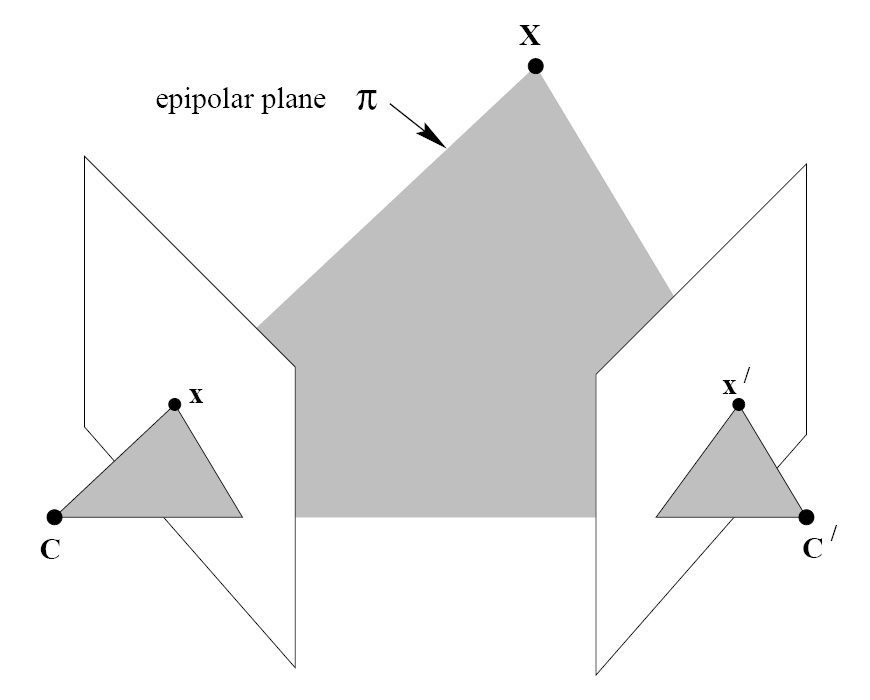
\includegraphics[width=.5\textwidth]{images/chap8/point_correspondence_geometry}

The line from $C$ to $C'$ is the \textbf{baseline}, the plane $\Pi$ containing $\mathbf{X}, C, C'$ is called \textbf{an epipolar plane}. (For each point we have one, except if they are on the same plane of course).

\textbf{Constraints on $x'$ given $x$:} \begin{itemize}
    \item $\mathbf{X}$ must lie on optic ray connecting $C$ and $\mathbf{x}$.
    \item $\mathbf{x'}$ must lie on the projection $\mathbf{l}'$ of this optic ray in $C'$
    \item This projection is called epipolar line corresponding to $\mathbf{x}$
\end{itemize}

\subsection{Epipolar planes and lines}

\begin{itemize}
    \item Baseline intersects the imageplane in epipoles $e, e'$
    \item Any plane $\Pi$ containing the baseline is an epipolar plane
    \item Intersections of $\Pi$ with the image planes are epipolar lines $l,l'$
    \item Moving a scene point $\mathbf{X}$ up or down, rotates the epipolar plane around the baseline
    \item All epipolar lines in one view, intersect at the corresponding epipole
\end{itemize}

\subsection{Fundamental matrix}

Denotes the relationship between points and their epipolar lines:

\textbf{Theorem}

Given $P, P'$, there exists $F \in \mathbb{R}^{3\times 3}$, s.t., $\mathbf{l}'$ for $\mathbf{x}$ is given by $$\mathbf{l}' = F \mathbf{x}$$, a pair of correspondences satisfies $$\mathbf{x'}^T F \mathbf{x} = 0$$,

$F$ is called the \textbf{Fundamental matrix} for the two views and can be estimated by correspondences alone.

\textbf{Properties:} \begin{itemize}
    \item $F$ for $(P,P')$, then $F^T$ for $(P',P)$ (\textbf{transpose correspondence equation)}
    \item The epipole $\mathbf{e'}$ is the left nullspace of $F$, i.e., $\mathbf{e'}^T F = 0$ and $F \mathbf{e} = 0$ (\textbf{all epilines contain the epipoles}), these equations \textbf{are used} to compute the epipoles once F is found
    \item $F$ has rank 2 (only the first two diagonal values are not zero)
    \item $F$ has \textbf{7 Degrees of Freedom}
\end{itemize}

\subsection{Computing the fundamental matrix for camera pairs}

1. Given $\mathbf{x}$ compute $\mathbf{X}_W$ which projects to $\mathbf{x}$. Using the pseudo-inverse we can find such a point using $$\mathbf{X}_W = P^+ \mathbf{x}$$

2. Project $\mathbf{X}_W$ into the second image using $P'$

3. Using the previously discussed property, we know that the epiline connects the epipole $\mathbf{e'}$ with $P'\mathbf{X}_W$, $$\mathbf{l'} = [\mathbf{e'}]_\times P' \mathbf{X}_W = \underset{=F}{\underbrace{[\mathbf{e'}]_\times P' P^+}} \mathbf{x}$$

4. The epipole $\mathbf{e'}$ is the projection of $P'C_w$ of the camera center of the first camera in world space, defined by $PC_W = 0$

\subsection{Pseudo-inverse of the projection matrix}

Using the SVD: $P^+ = V \Sigma^+ U^T$, $\Sigma^+$ constructed from $\Sigma$ taking the reciprocal of the diagonal values and then transposing the matrix. For projection matrices $n < m$ and we get $\Sigma^+$ as a right-inverse of $\Sigma$, thus $$PP^+ = U\Sigma V^T V\Sigma^+ U^T = I_3$$.

\subsection{Solutions for Fundamental matrix}

\textbf{Important} to not confuse $n<m$ and $n>m$.

$n>m$: System is over determined, usually no solution. Pseudo-inverse $\hat{x} = A^+ b$ computes $\hat{x}$ s.t. the distance from $b$ is minimized: $$\hat{x} = \mathrm{argmin} ||Ax - b||^2$$.
Pseudo-inverse finds the best approximate solution to $Ax = b$ and is a \textbf{left-inverse}.

$n<m$: Situation for the fundamental matrix. System is \textbf{under-determined}, infinitely many solutions. Pseudo-inverse $\hat{x} = A^+ b$ computes $Ax = b$ which minimizes \textbf{the norm of} $x$: $$\hat{x} = \mathrm{argmin}_{Ax = b} ||x||$$.
I.e., computes a minimum norm solution for $Ax = b$. The pseudo-inverse is a \textbf{right-inverse}.

\subsection{Summary for fundamental matrix}

For projections $P,P'$, $F = [e']_\times P' P^+$ with $e' = P'C_W$ and $PC_W = 0$. If translation and rotation parameters are known: $C_W = T^{-1} R^T \rectmat{0\\0\\0\\1}$

\subsection{Pure translational motion}

Epipole is fixed, points move along lines radiating from the epipole, hence $F = [e]_\times = [e']_\times$.

\textbf{Compact notation for a pinhole camera}: $P = K[R|t]$.

Show the previous property formally: Choose parameters $P = K[I | 0], P' = K[I | t]$. Then $P^+ = [K^{-1} \ 0]^T$ and $P'P^+ = KK^{-1} = I_3$, hence the result is \textbf{independent of translation}.

Also $C' = [-t \ 1]^T$ in world coords, thus $\mathbf{e} = K[I|0] [-t | 1]^T = -K t = Kt$ and $\mathbf{e'} = K[I|t][0 \ 1]^T = Kt$ and we have $\mathbf{e} = \mathbf{e'}$.

This way it is clear that the first statement holds.

\textbf{Horizontal motion}

Parallel to x-axis: epipole at $\mathbf{e'} = [1 \ 0 \ 0]^T$ and thus $$F = \rectmat{0 & 0 & 0\\ 0 & 0 & -1 \\ 0 & 1 & 0}$$ and the correspondence relation reduces $x' F x = 0$ to $y = y'$, along horizontal lines.

\subsection{Estimating F}
Given $n$ correspondences, for the $i$-th correspondence we get the constraint: 
$$0 = \mathbf{x'}_i F \mathbf{x}_i = [x'_i \ y'_i \ 1] \rectmat{f_{11} & f_{12} & f_{13} \\ f_{21} & f_{22} & f_{23} \\ f_{31} & f_{32} & f_{33}}[x_i \ y_i \ 1]$$ which resolves in the equation $$x_ix'_i f_{11} + y_ix'_i f_{12} +x'_i f_{13} + x_ix'_i f_{21} + y_ix'_i f_{22} + y'_i f_{23} + x_i f_{31} + y_i f_{32} + f_{33}$$ and from which we get the following system:

$$[x_ix'_i \ y_ix'_i \ x'_i \ x_iy'_i \ yiy'_i \ y'_i \ x_i \ y_i \ 1] \rectmat{f_{11} \\ f_{12} \\ f_{13} \\ f_{21} \\ f_{22} \\ f_{23} \\ f_{31} \\ f_{32} \\ f_{33} \\} = 0$$, the solution is again the rightmost column of $V$ in the SVD.

\textbf{Enforce Rank-2 constraint:} To get well-formed $F$ it must be rank 2. Compute the SVD $F' = V \Sigma V^T$ and set the last diagonal value to $0$, $F$ is then the closest to $F'$.

\textbf{Increase robustness using RANSAC:} Remove outliers using RANSAC for accurate estimation. Sufficient to estimate $F$ are \textbf{eight} sample points. "Inliers" are the feature matches satisfying the epopolar constraint given a threshold, i.e., $x' F x \leq \epsilon$.

\textbf{Summary:}

\begin{itemize}
    \item Compute feature matches (SIFT)
    \item Simple: Build large system, solve for $F$, enforce rank two constraint
    \item More robust: use RANSAC
\end{itemize}

\section{Perspective, affine and metric reconstruction}

\textbf{Projective ambiguity}: Given correspondences and assuming we reconstructed $P,P'$ and some world coordinates. Given \textbf{any} homography of the world, applying it onto the world coordinates and the projections (computing new cameras), we get the \textbf{same fundamental matrices} for the new and the old projections!

I.e., both reconstructions lead to \textbf{exactly the same correspondences}. \textbf{Mathematical limit of what we can reconstruct from correspondences alone!}

This is \textbf{projective reconstruction}.

\subsection{Affine reconstruction}

Better, as parallel lines map to parallel lines, angles are not necessarily correct.. In order to do this, we need to get rid of \textbf{projective ambiguity}. One possibility is, to identify the \textbf{plane at infinity} $\pi_\infty$.

\textbf{Plane at infinity:} Can be identified, e.g., from correspondences of \textbf{three vanishing points} detected in both images. (For instance 3 sets of parallel lines).

\subsection{Metric reconstruction}

Correct reconstruction \textbf{up to similarity} transformations (parallel lines and angles correct), but the scene might be scaled uniformly.

\textbf{Scaling ambiguity:} Segment with known absolute length must be identified (in both images).

In order to do \textbf{metric reconstruction}, we need to identify \textbf{absolute angles} (complex and not discussed!). Short: Find intrinsic parameters $K$, for which we need to compute the \textbf{Image of the Absolute Conic} (IAC), which can be described by $3\times 3$ symmetric matrix $\omega = (KK^T)^{-1}$. If $\omega$ is known, $K$ can be recovered by inverting $\omega$ and computing \textbf{Cholesky decomposition}. (The last part is not that important I guess).

\textbf{Constraints to pick from while finding $\omega$:}

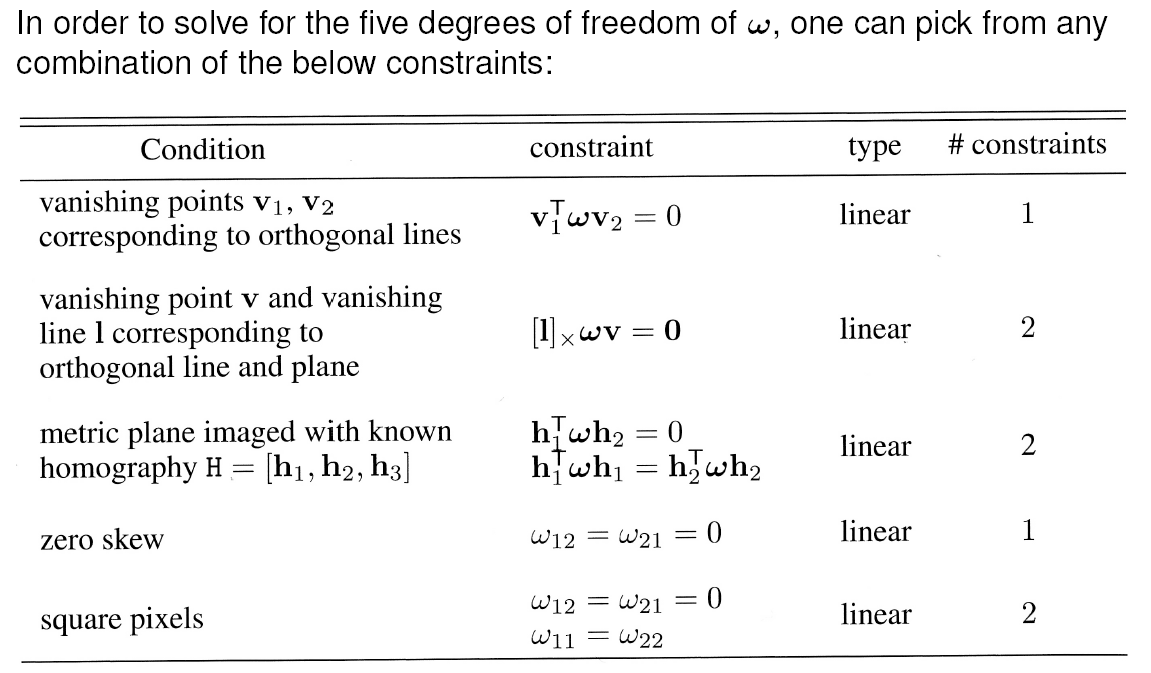
\includegraphics[width=\textwidth]{images/chap8/omega_conditions}

\section{Pose estimation : the essential matrix}

\textbf{Essential matrix:} Specialization of fundamental matrix to the pre-calibrated case where $K$ is known (hence we have \textbf{metric reconstruction}).

Under assumptions \textbf{square pixels, center of projection is center of image} we only need to calibrate the \textbf{magnification} of $K$ (focal length times pixels per meter).

\textbf{Definition:} Defined in terms of homogeneous coordinates. From a corresponding pair we get the correspondence: $$K^{-1} x = \hat{x} \leftrightarrow \hat{x}' = K'^{-1} x'$$.

The defining equation for $E$ is the correspondence constraint $\hat{x}'^T E \hat{x} = 0$. Thus, $E = K'^T F K$, and $E$ has rank two.

\textbf{Derivation from a pair of cameras:} Given a \textbf{normalized} camera pair $P = [I|0], P' = [R|t]$, we get for $E$: $$E = [e']_x P'P^+ = [[R|t][0 \ 0 \ 0 \ 1]^T]_\times [R|t][I \ 0]^T = [t]_\times R$$

Not going into detail for the decomposition..

\section{Triangulation: structure from motion}

We have two cameras $P,P'$ and correspondences. We want to find a 3D world point $PX = x$ and $P'X = x'$. Correspondence measurements usually have errors, but we can compute it (non-error free) by minimizing the \textbf{reprojection error}:

$$E(X) = \sum\limits_{i=1}^n ||PX - x||^2 + ||P'X - x'||^2$$.

\textbf{Direct linear triangulation:} $X$ can be recovered as solution to $AX = 0$:

$$A = \rectmat{x(p^3) - p^1 \\ y(p^3) - p^2 \\ x'(p'^3) - p'^1 \\ y'(p'^3) - p'^2}$$

Notes: \begin{itemize}
    \item Generalizes easily to multiple views
    \item Easy to implement
    \item Not nice mathematically: not proj. invariant
    \item Affine invariant if last coord. is forced to be zero
\end{itemize}




\include{09}

\end{document}